%& -jobname=A_Familia_de_Serrinha
%%%%%%%%%%%%%%%%%%%%%%%%%%%%%%%%%%%%%%%%%
%  A Familia de Serrinha
%  
%  Livro Histórico de 1929 que fala sobre a povoação do semi-arido baiano
%	
%
%%%%%%%%%%%%%%%%%%%%%%%%%%%%%%%%%%%%%%%%%

%------------------------------------------------------------------------------------
%	Pacotes e outras configuracoes
%------------------------------------------------------------------------------------

\documentclass[12pt]{book} 

\usepackage[portuguese]{babel}


\usepackage[table,xcdraw]{xcolor}
\usepackage{xcolor,lipsum} % Required for specifying colors by name
\definecolor{ocre}{RGB}{51,102,0} 
\definecolor{lightgray}{RGB}{229,229,229} 
\usepackage{bookmark} %marcadores

% Font Settings
\usepackage{avant} % Use the Avantgarde font for headings
%\usepackage{times} % Use the Times font for headings
\usepackage{mathptmx} % Use the Adobe Times Roman as the default text font together with math symbols from the Sym­bol, Chancery and Com­puter Modern fonts

%\usepackage{fancyhdr}
\pagestyle{plain}


\usepackage{makeidx} %cria indice.

\usepackage{float}
\usepackage{geometry} %altera margens/dimensoes de uma pagina

% MATHS PACKAGE
\usepackage{amsmath,tikz}
\usetikzlibrary{matrix}
\newcommand*{\horzbar}{\rule[0.05ex]{2.5ex}{0.5pt}}
\usepackage{calc}



% serve pra colocar texto sem formatação (codigo)
\usepackage{verbatim}

% Bibliography
\usepackage[style=alphabetic,sorting=nyt,sortcites=true,autopunct=true,babel=hyphen,hyperref=true,abbreviate=false,backref=true,backend=biber]{biblatex}
\addbibresource{bibliography.bib} % BibTeX bibliography file
\defbibheading{bibempty}{}


\makeindex

\begin{document}


%------------------------------------------------------------------------------------
%	CAPA
%------------------------------------------------------------------------------------
%\thispagestyle{empty}
%\topmargin=-20mm
%\hoffset=-20mm
%\voffset=-20mm

%usando newgeometry pra alinhar a imagem da capa.
\newgeometry{left=5mm,right=5mm,top=2mm,bottom=5mm}
\begin{figure}

\centering
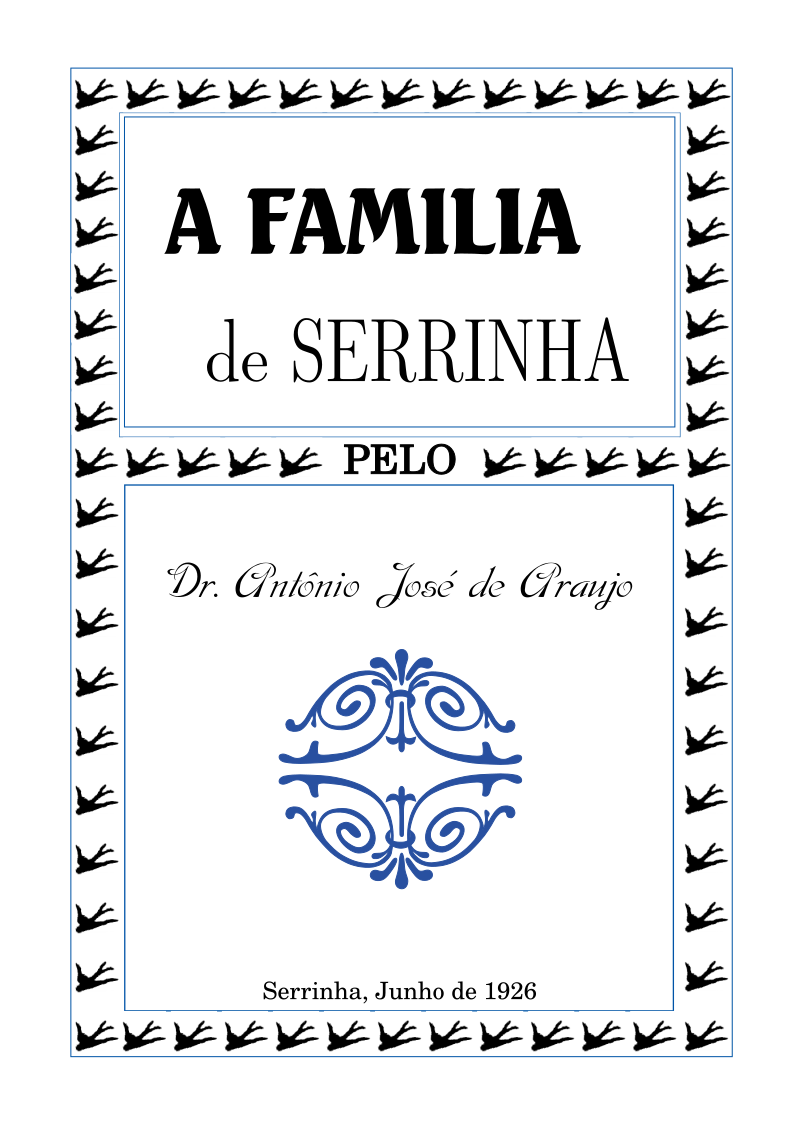
\includegraphics[scale=0.95]{capa.png}

\end{figure}
\restoregeometry
%------------------------------------------------------------------------------------
%Informações Autorais
%------------------------------------------------------------------------------------

\thispagestyle{empty}


\onecolumn
\newpage
\thispagestyle{empty}
\begin{center}
\vspace*{5cm}
\Huge{\textbf{A Família de Serrinha\\}}
\vspace*{3cm}
\huge{\textbf{Dr. Antônio José de Araújo\\}}
\vspace*{7cm}
\huge{\textsc{Typ. do "O Serrinhense"}}
\end{center}

\newpage
\thispagestyle{empty}
%\noindent Copyright \copyright\ 1929 Dr Antônio José de Araújo\\ % Copyright notice
%\small
\noindent \textsc{A Família de Serrinha}\\\\
\noindent \textsc{Originalmente Publicado em Junho de 1926 por:}  \textit{Dr Antônio José de Araújo}\\
\noindent \textsc{Juiz de Direito de Jacobina} \\ % License information
\noindent \textsc{Publicado por:} \textit{Typ. do "O Serrinhense"}\\ 
\newline
\noindent {Reedição realizada por Eder Carneiro}\\ 
\noindent Fonte (Latex) em \url{https://github.com/escarneiro/famSerrinha}\\ 

%------------------------------------------------------------------------------------
%	Índice
%------------------------------------------------------------------------------------
\tableofcontents
%------------------------------------------------------------------------------------
%	Capitulos
%------------------------------------------------------------------------------------

%\chapterimage{sisal\_pb.jpg} % Chapter heading image
\chapter{O Povoamento do Sertão}

%\section*{}
Descoberto o Brazil em 1500 pelo almirante Pedro Alvares Cabral, que delle tomou posse
em nome da Corda Portugueza, não pensou esta senão em utilisar-se das suas muitas riquesas naturaes de mais facil disposição, sem cuidar de occupal-o, colonisal-o e conduzil-o ao banquete da civilisacão.

Somente trinta e quatro annos depois, em 1534, é que, aguçada a ambição dos demais
povos europêos, e a della mesmo, resolveu dividil-o em capitanias de cincoenta leguas de littoral, distribuindo-as por subditos capazes de firmar nellas o seu dominio. A da Bahia, do Tio Jequiriçá ao S. Francisco, coube a Francisco Pereira Coitinho, que se deu pressa em aproveital-a, fundando o seu primeiro estabelecimento, no logar Victoria, encostado á Graça, onde já encontrou o seu patrício Diogo Alvares Correia, o caramurú, que ahi naufragara  em 1510, e  tendo sido bem acolhido pelos naturaes do paiz, recebera por mulher, segundo  os usos  destes a Catharina Paraguassú.

Morto Pereira, que pouco ou nada pudera fazer pelo desenvolvimento da sua capitania, e paralisada senão abandonada, por muito tempo a obra de colonisação, resolveu a Coroa Portugueza avocar as capitanias, entregando-as em 1548 a Thomé de Souza, a quem nomeou Governador Geral do Brazil com séde na Bahia.

Esse foi o passo mais  seguro, mais efficaz e mais decisivo, para a definitiva conquista e  consequente povoamento da Bahia e seus sertões.  Arrojados exploradores já haviam se internado bastante e chegado ás margens do alto S.Francisco, espalhando noticias phantasticas sobre as suas riquezas em prata ouro e pedras preciosas, que, si outro effeito não tiveram, o de restimular ao menos a gente portugueza não se lhes pode negar. A nomeação de Thomé de Souza foi de certo consequencia de uma dessas phantasias, a de  Guilhen\footnote{Filipe Guilhem, espanhol que era padre/boticário/mensageiro e muito serviu à coroa Portuguesa.}, %Felipe Gulhem 
que para Portugal escrevia a miúde, mandando contar  cousas do arco da velha, iriadas, como este, eram ellas.

E por o ter sido é que veio completamente apparelhado para uma obra completa, duradoura, sem desfallecimentos. Não podia ter esquecido, como não esqueceu, um factor na epoca  de grande monta, o frade, sobretudo o jesuita, muito mais inteligente, illustrado e experimentado e por isso mesmo mais  pratico e efficiente do que outro qualquer.

Mal fundada a Villa, no mesmissimo logar  onde  está hoje  a cidade, que tem se estendido bastante, um pouco distante da  primitiva agora por ella absorvida, que, por isso mesmo, ficou chamando-se villa velha, ou arraial do Pereira, actualmente Victória, começou a obra de cathechese e colonisação. Por um lado os frades, e  por outro  destemidos exploradores, que de nada se arreceiavam, puseram-se em demanda do sertão, que palmilhavam, a principio o mais baixo, depois o do meio ou centro, por fim o alto. Os rios foram os caminhos que tiveram. Quando chegaram ás suas cabeceiras e as grandes vastidões territoriaes ainda se estendiam por ellas afóra,  começaram a abrir trilhos que os pusessem em communicação com os rios de curso mais longo que os contornavam alem, ou mais facilmente unissem os logares que melhor se  affeiçoassem ao genero de sua actividade, agrícola, pastoril ou mineira. Surgem as primeiras aldeias de naturaes do paiz sob a direcção espiritual do frade, apprecem as mais antigas fazendas de criar, despontam os sítios da lavoura. Ao lado do frade duas figuras de grande relevo, como que representando as demais, se levantam.

São Garcia d'Avila e Antonio Guedes de Britto,  os dois maiores proprietarios de terras na capitania da Bahia, troncos respectivamente das casas da Torre e da Ponte. Os seus curraes se enchem de gado, como se enchem os curraes de muitos outros sertanistas de destaque, e vê-se florescerem as aldeias de S. Antonio (Aratuhype), ao sul, Tatuapara, S. Pedro e S. André, ao norte.

Quando em 1624,cento e vinte quatro annos depois da descoberta do Brazil e setenta e seis da fundação da cidade do Salvador, Bahia de todos og Santos, os hollandezes quizeram fazer da terta bahiana sua preza, já o nosso littoral estava cortado de estradas e cheio de aldeias largamente povoados de indios pacificados e pelo baixo sertão ostentavam-se innumeros estabelecimentos agricolas e pastoris.

Tão notavel era já a obra do povoamento, que a esse tempo se descriminavam no reconcavo diversas freguezias, como fossem N. S, da Purificação de Santo Amaro, S. Bartholomêo de Pirajá,  N. S. da Conceição de Itapuan, Bom Jesus da Veneravel Cruz de Itaparica, N. S. da Piedade de Matuim e N. S. da Ajuda de Jaguaripe. Eram logares todos esses fartamente povoados. O sertão que até então se resentira
 desse beneficio, infestado que ainda se achava de indigenas refractarios a toda e qualquer tentativa de cathechese e pacificação. Mas ainda assim,  com poderoso auxilio de naturaes  do paiz, que se haviam deixado domesticar, não foi difficil resistir aos invasores, que aliás somente trinta annos  depois, em 1654, foram de todo expulsos.
 
 A luta retardou por muito tempo a obra da colonisação, mas não  a estagnou de todo. Durante ella vio-se surgirem novas aldeias, missão da Saúde, hoje cidade  de Itapicurú, S.S. Trindade de Massacará e outras. Uma vez terminada porem, redobraram-se os esforços e, já não havendo inimigos externos a combater, cuidou-se exclusivamente do inimigo interno, o indio, que senhor ainda de todo o sertão, trazia em sobresaltos as nascentes povoações, que, por elles atacadas inopinadamente, eram muitas vezes devastadas ou destruidas.
 
 A luta agora não foi menos cyclopica. Organisaram-se bandeiras, repetiram-se as entradas, abriram-se  estradas e vencidos definitivamente em 1693 os ultimos recalcitrantes, os Maracás, ficou firmado o domínio dos portuguezes, que desde então passaram a  gozar com toda tranquilidade as terras que prodigamente lhes foram dadas em sesmaria, os curraes que nellas estabeleceram, as fazendas que fundaram, os sitios  que estabeleceram. Criavam-se as primeiras villas, Jaguaripe em  1697, Cachoeira e S. Francisco de Sergipe do Conde em 1698. Affloraram diversas missões no sertão,
  N. S. das Neves (Sahy)\footnote{Atual Senhor do Bonfim-BA} % 				Senhor do Bonfim-BA
 em 1697, N. S. do "O" (Sorobabé)\footnote{Atual Ilha Surubabel em Rodelas-BA}%		Zorobabel ou Surubabel, em Rodelas-BA
 , S.  Francisco (Curral dos Bois\footnote{Atual Gloria-BA})%		Gloria - BA 
  em 1702, N. S. da Piedade (Hunhunhús)\footnote{Atual Santa Maria da Boa Vista - PE} % Sta Maria da Boa Vista - PE
  Bom Jesus (Jacobina), %		 			Jacobina
  N. S. dos Remédios (Pontal)\footnote{Ilha do Pontal, BA/PE} % 			Ilha do Pontal BA/PE (Juazeiro)
  em 1705, N. S. de Brotas (Joazeiro) %	Juazeiro - BA
 em 1706. O povo, descansado dos  hollandezes e já sem se encommodar muito com os indeios, começou a espalhar-se por todo o sertão, em procura de mineraes ou de logares onde  mais folgadamente podesse entregar-se a exploração de industria pastoril.
 
 Agua Fria e  Inhambupe tomaram impulso e fizeram-se freguezias, em 1718. Descobriram-se por esse tempo as minas de ouro de Jacobina e Rio de Contas. Para ellas affluiram mineradores. Formaram-se logo, ao seu redor, sitios de Lavoura, Coqueiros, Lagôa, etc.
 
 A noticia chegou celere aos ouvidos dos  homens do governo. Tratou-se de criar  villas para amparar o fisco. Um desembargador foi destacado para esse fim: adoeceu em caminho, ahi pelo sertão dos Tocós, e voltou. Não foi possivel que um outro se  incumbisse dessa tarefa. Lembrou-se então o governador do coronel Pedro Barbosa Leal, filho do celebre sertanista Francisco Barbosa Leal, sertanista como  seu pae, e foram fundadas as villas de Jacobina em 1720, e Rio de Contas em 1724, as primeiras villas do sertão bahiano, e ligadas por uma estrada. Mas as suas  situações  não agradaram. Em 1724 mudou-se a de Jacobina  da Missão do Sahy, onde ficava, para a Missão do Bom Jesus,  onde ainda hoje está, e em 1725 a do Rio de Contas da margem do Bromado, onde se levantava o planalto  onde desde então florece.
 
 \newpage Ligadas as duas villas entre si, foram logo unidas á cidade do Salvador, Bahia de todos os Santos, por estradas traçadas por cima das velhas picadas, dos trilhos primitivos. O surto nunca mais foi detido.\label{surto}
 
 Uma dessas  estradas, aberta por Garcia d'Avila e outros,  grande criadores de gado no alto sertão, entre os  annos de 1654 e 1698, para conducção de suas boiadas e rectificada e melhorada pelo coronel Pedro  Barbosa Leal em 1729, quando fundou a villa de S. Antonio de Jacobina,  cortava o sertão  dos Tocós, também chamado de Pindá, onde ficavam o arraial de  Agua Fria e as fazendas de Sacco do Moura, Serrinha, Tambatá, Massaranduba, Pindá, Cuyaté, etc. Em Serrinha, tomava ás direitas, pela fazenda  Raso, hoje villa Aracy, para Geremoabo e Pontal no rio S. Francisco, e  no tanque do Papagaio, adiante de Cuyaté, tomava ás direitas para Tiuba, ou Itiuba, como se diz hoje, e Joazeiro, no rio S. Francisco, as esquerdas para Jacobina. Serrinha, que em 1716 era simples logradouro da fazenda Tambutá, onde já morava Bernardo da Silva, passou em 1723 por compra que de suas terras e das terras do Tambuatá fez Bernardo da Silva aos antepassados da casa da Ponte, á sede da  fazenda, que deixou de ser Tambuatá para ser Serrinha, ficando Tambuatá como logradouro. Morto Bernardo, foi partilhada entre os seus herdeiros, que doaram algumas braças de terra, no local da casa da fazenda, a N. S. de Sant'Anna e ahi erigiram uma capella, que, concluida em 1780, foi em 1838, deseseis annos depois da  nossa emancipação  politica, elevada á cathegoria da  matriz da freguezia ahi então criada. A freguezia ficou annexada ao Termo da villa  de Purificação dos Campos, criada no anno anterior em substituição á villa de S. João Baptista de Agua Fria, então extincta, e só em 1876, por influencia e prestigio do inesquecivel capitão José  Joquim de Araujo, o popularissimo capitão Zezinho da Soledade, pae do autor destas linhas, gozou dos fóros de villa, e agora elevada a cidade.
 
 


%\chapterimage{pano-5.jpg} % Chapter heading image
\chapter{O Sertão dos Tocós}

 Em 1609 a penetração, que se havia encaminhado pelos rios - vias únicas de comunicação que então se podiam utilisar, inexistentes que eram as estradas - e atingindo as cabeceiras dos de curso menor, Joannes, Pojuca, Sabahuma, Inhambupe e Real, ganhou maiores extensões nos de maislonga carreira, Jequiriçá, Paraguassú, Itapicuru e São Francisco, principalmente São Francisco, traduzindo-se este facto em novas e mais vantajosas sesmarias, concedidas áquellesque nas conquistas arriscavam sua vida, fazenda e commodidades.
 
 O mestre de campo Antonio Guedes de Britto, bisavô  de  D. João de Saldanha, conde da Ponte, sertanista como seu pae Antonio Correia de Britto - o qual já havia tido muitas sesmarias e posteriormente  teria de haver várias outras mais importantes - por carta régia de 21 de Julho deste anno, 1609, obteve todas as terras existentes entre os rios Itapicuru e Inhambupe, nas cabeceiras das que já possuia nos nascentes dos rios Real  e Piagoay, e, para o sertão, mais dez léguas  medidas rumo direito com todas as pontas, enseadas, mattos, aguas e mais pertences (Felisbello Freire, Hist. Territorial do Brazil, pag. 28).
 
 Essa data  comprehende os então conhecidos por sertões dos Tocós, do Pindá  e do Tucano. Abrange os actuaes municipios de Queimadas, Tucano, Aracy (Raso), Coité, Serrinha e Riachão do Jacuípe, que, separados por pequenas distâncias entre si, se ligavam pela comunidade de interesses dos seus habitantes.
 
 Teve voga no seu tempo esta quadra, de antiguidade quasi secular, demonstrativa não só do espírito folgasão  de quem a compoz, senão ainda do desapontamento deparado  por quem esperava talvez somente goso bem estar nas incontinencias de um temperamento pronunciadamente andêjo, em displicencia por esses logares.
 \begin{verse}
 	\hspace{4em}Serrinha não Serra pao grosso,\\
 	\hspace{4em}Coité não dá selamim,\\
 	\hspace{4em}Raso não tem fundura,\\
	\hspace{4em}Queimadas não nasce capim.\\
 \end{verse}

 
 É uma zona, cuja fertilidade incontestavel é entretanto altamente prejudicada pela escassez dos rios perennes, pela inconstancia das chuvas, pelo flagelo das secas periodicas e exterminadoras, e que aliás foi promptamente povoada não só por ser trajeto obrigado da estrada da Bahia ao S. Francisco e ao Piauhy, por onde desciam as boiadas, como também por se prestar, na época, admiravelmente, á criação, hoje desfavorecida pelo augmento da lavoura.
 
 Doada, como todas as outras terras , com a clausula de occupação e cultivo, em prazo mais ou menos curto, o seu  donatário de espaço a espaço, com intermittencia de uma, duas, tres  e mais legoas, segundo a maior ou menos feracidade  dos terrenos e a maior ou menor possibilidade de captação das aguas das chuvas, fazia um curral,  ponha-lhe ao lado uma casinha e um cercado, ahi collocava uma familia de agricultores, facilitando ao seu chefe tudo, o escravo para o trabalho e o gado para criar, e cobrando-lhe renda modicissima, que raramente ultrapassava doze  mil réis e não pouco baixava a quinhentos réis por anno. E assim tinha fundado um  estabelecimento agrícola e pastoril, tinha feito um sítio. O rendeiro tomava conta desse sitio na esperança  de fazer-se proprietário delle por compra, e isto foi o que sempre aconteceu, se não logo, de certo mais tarde, quando já não  foram de temer nem as invasões dos estrangeiros - que demandavam homens e armas para defeza do paiz, nem os ataque sdos indios - que embaraçavam o desenvolvimento dos estabelecimentos agricolas.
 
 Encerrado o cyclo daquelas, posto termo a estes, o sentimento de propriedade despertou e o rendeiro, ja aproveitando melhor o seu  trabalho, poude fazer-se, por compra, senhor do solo, quasi todo em poder das casas influentes e poderosas.
 
 O mais antigo documento de alienação de Terras no sertão dos Tocós, de que temos noticia, é de 1716. É uma escriptura  publica de venda, que d. Izabel Maria Guedes de Britto, viúva do coronel Antonio da Silva Pimentel, passou na cidade do Salvador, Bahia de todos os Santos, em 31 de Maio, ao capitão Antonio Homem da Affosenca Correia,  morador nos campos do termo  da villa de Cachoeiram dos sitios  Massaranduba, Serra  Grande e Dois Irmãos, herança do seu fallecido pae Antonio Guedes de Britto, por 1:500\$000\footnote{A moeda do tempo era o "réis". Leia-se aqui o valor de "mil e quinhentos mil-réis" (ou mirréis)}
 
 A divisa desses sitios era a seguinte: começava
 onde fazia meio certo a estrada da fazenda Massaranduba,
 onde estavam as casas do capitão João Alvares Filgueiras, para o “Tambuatá, onde morava Bernardo da Silva, e dahi, como pião, corria ramo direito para a parte do Nascente até chegar ao Morrinho que está entre o Saco Grande e a fazenda da Serra e Serrinha e elle corria direito á nascença do riacho da Tapera
 e por elle abaixo, com todas as voltas e e enseadas até as Capueiras que fizeram no rio Salgado, que, sendo o mesmo da dita Papera, em sua nascença lhe chamam Salgado, embaixo, nas capueiras, cincoenta braças abaixo dellas, seguia para a parte do Norte, rumo direito á quarta parte do norte, buscando as
 catingas até endireitar ou emparelhar com a casa do sitio chamado Dois Irmãos, e dahi seguia para diante com o mesmo rumo até se encher da meia legua e nesta forma se dividia então por esta parte, ficando bem como o sitio do Salgado, aonde morava Gaspar Pinto, para se medirem e demarcarem pelas partes
 do Poente. Tornava ao primeiro pião da estrada, que estava entre o Tambuatá e Massaranduba, e delle corria rumo direito para a parte do Poente até ficarem de dentro, para a parte da Massaranduba, do dito rumo à chegar á primeira baixa, vindo do riacho de Subaé, á mão esquerda, pela estrada que vinha para à Massaranduba e depois de salvar esta dita legua ia seguindo o mesmo rumo em que viesse até encher a meia do rumo que corria para as catingas com que se dividiam com o sitio Dois Irmãos e de um e outro rumo, onde findassem, se botaria o travessão pela parte da catinga.
 
 Só sete annos depois, em 1723,por escriptura publica passada na Bahia e pousadas de D. João de Mascarenhas, este e sua mulher d. Joanna da Silva Guedes de Britto, em notas do tabelião Manoel Affonso da Costa, venderam a Bernardo da Silva, morador no sertão dos Tocós por 2:200\$000, á vista, as terras do sertão dos Tocós e nellas um sítio chamado Serrinha, que houveram por titulo de herança de seu pae e sogro o coronel Antonio da Silva Pimentel, o qual sítio de terra, assim chamado a Serrinha, confronta e demarca por uma parte com terras delles vendedores, e sitio em que está de renda Gaspar Pinto, buscando o taboleiro que vae para a catinga onde morou Antonio Gonçalves e demarcando ao meio com o Saco do Moura, donde corre rumo à tapera do Cypriano, de lá cortando á entestar e demarcar com terras de Francisco de Sá Peixoto, de outra parte com rumo á partir com terras do cel. Antonio Homem, por outra parte ainda,corre direito o rumo à partir com terras de Manoel Carlos Lima, e deste corre rumo direito à entestar e partir com o Saco dos Tapuyo buscando a lagoa do Genipapo, correndo o rumo
 direito a entestar com terras do dito Francisco
 de Sá Peixoto.
 
 Eis  que era o sertão dos Tocós em 1723. Uma porção de sitios de lavoura e criação, a pequena distancia uns dos outros, um dos quaes Serrinha, hoje cidadem por um lado se limitavacom os sitios Massaranduba, Serra Grande e Dois Irmãos, de propriedade do coronel Antonio Homem da Fonseca Correia, que aliás não morava nelles, por outro lado com o sitio
 Salgado, propriedade de D. João Magicarenhas
 mulher d. Joanna, que o tinha arrendado a Gaspar Pinto, por outro lado com o sitio de Manoel Carlos de Lima e finalmente por outro lado com o sitio de Francisco Ge Sá Peixoto.
 
 Foi, pois, Bernardo da Silva, depois do mestre de campo Antonio Guedes de Britto, seu, genro coronel Antonio da Silva Pimentel e d. Joanna da Silva Guedes de Britto, flha deste casada
 em primeiras nupcias com D. João Mascarenhas e em segundas com D. Manoel de Saldanha, senhores primeiros de todo o sertão dos Tocós e de grandes tratos de terras nos sertões do Tucano, rio de S. Francisco, Jacobina, Itiuba, Rio de contas e Rio Pardo -  o primeiro e unico proprietario do sitio Serrinha, que, por sua
 morte passou a seus filhos e genros e hoje se acha na posse e domínio de seus tetranetos e filhos destes.
 
 Conforme se vê da escriptura de venda dos sitios Massaranduba. Serra Grande, Dois Irmãos, passada em 1716 por D. João de Mascarenhas e sua mulher D. Joanna ao capitão Antonio Homem, ddesde esse tempo Bernardo da Silva era morador no Tambuatá, terras do sitio Serrinha, como o capitão João Alvares Filgueiras o era em Massaranduba, onde tinha casas, e Gaspar Pinto no Salgado.
 
 Bernardo da Silva, portanto, sete annos antes de comprar o sitio Serrinha, já morava nelle logar Tambuatá, pagando renda,
 e todo esse sertão, desde 1698, segundo se vê de uma representação dirigida ao governo portuguez, estava povoado de moradores brancos com suas fazendas. (Inv. dos doc. rel ao Brazil no arch. de Mar. e Ultramar de Lisbõa, org. para a Bib. Nac. por Eduardo de Castro e Almeida, pag. 21)
 
 Então o caminho de Bahia a Jacobina e S. Francisco, por Agua Fria, até 18 ou 20 legoas de Bahia, tinha 3 freguezias: Rosario do Porto da Cachoeira, S. Gonçalo dos Campos e São José das Itapororocas, — e duas capellas,— N. S. da Conceição e N. S. do Desterro, - com suas igrejas e d'ahi pra cima, passando embora pelas povoações dos Tocós e do Pindá com bastante moradores, não tinha uma só Igreja, uma só freguezia, mas tão somente uma capella curada em Jacobina.
 
 Em 1731, oito dam depois da compra de Serrinha por Bernardo da Silva e trinta e três da representação a que vimos de nos referir, quando o mestre de campo Joaquim Quaresma Delgado, encarregado por portaria de 11 de Janeiro de percorrer os districtos de mineração da capitania da Bahia escreveu os seus celebres roteiros de Bahia a Jacobina, de Jacobina a Minas do Rio de Contas e de Minas a Bahia, a situação desses sertões só havia mudado em se haver criado em 1718 uma freguezia em
 Agua Fria e ahi erigido uma igreja e em 1727, com o pelourinho e a força, installado uma vila.

\chapter{O Tronco da Família}

Em sua rota de Passagem ou Trapiche Velho, nos arredores da cidade do Salvador, Bahia de todos os Santos, a Jacobina, o mestre  de campo Joaquim Quaresma Delgado, palmilhara a estrada das boiadas, cujo traço foi depois seguido pela ferrovia da Bahia a Joazeiro. Pequenos ranchos, poucos moradores, povoados insignificantes, foi tudo quanto encontrou. Em todo seu peregrinar só vio um engenho de assucar. Pojuca foi o lugar venturoso que o ostentou. Em todos os outros, alguns dos quaes hoje vilas mais ou menos importantes como Matta de São João, Catu e mesmo Pojuca, cidades de muita actividade e progresso, por exemplo, Alagoinhas e Serrinha, não notou senão ranchos, casas raras e e diminutissimo numero de habitantes. Faziam excepção a esta regra, Agua Fria com a sua Igreja de S. João Baptista de Agua Fria e as mais casas distantes da estrada a parte do oeste coisa de meia legua. Serrinha logar de bastantes casas com seus moradores e fazenda de gado, e Jacobina, villa de uma rua arruada leste oeste, com casas de uma banda e da outra.  Jacobina foi villa em 1724. Agua Fria já era freguezia desde 1718, e villa á partir de 1727, quando a carta regia de 24 de Abril a elevou a essa dignidade, desmembrando-a de Cachoeira, que foi creada villa em 1689. Serrinha lhe pertencia, mas como uma simples fazenda de gado, de propriedade de Bernardo da Silva, criador abastado e chefe de numerosa prole. Só por morte de Bernardo, a qual devia ter ocorrido pouco antes de 1763, senão n'este anno, é que se pensou em érigil-a em Arraial, embora já tivesse, desde muito tempo, a sua capella sob a invocação de Senhora Sant'Anna.

Em um documento de 1763 se fallou no "sitio de Senhora Sant'Anna de Serrinha"; em outro de 1775 se fallou tão somente "sitio Serrinha", mas em 1814 já se fala, no "arraial da Serrinha". Serrinha, portanto só foi arraial depois de 1750, quando foi concluida a capella, que ainda hoje é a Matriz da freguezia, O arraial conseguintemente não é obra de Bernardo; mas de seus filhos e genros. Foram estes senão os iniciadores, pelo menos os concluidores da construção da igreja, que ainda hoje é a mais sumptuosa das suas construções, toda de pedra e cal que é. É crível que o impulso poderoso tivesse partido de sua viuva, Maria do Sacramente, fortemente amparada por seus filhos; Pe.Prudente e Maria da Purificação, esta solteira, d'uma piedade rara, de uma vida sem um  minimo deslise, toda virtude e bondade. Nenhuma duvida existe sobre a personalidade de Bernardo da Silva, de sua mulher Maria do Sacramento e seus filhos. Eram elles em 1731 os moradores das "bastantes casas", bem como os proprietários da fazenda de gado, que o mestre de campo Quaresma, de viagem de Bahia para a villa de Jacobina, encontrou em Serrinha. Não sei se elles eram portuguezes, ou tão somente descendentes de portuguezes.

Talvez Bernardo da Silva, seja filho, ou mesmo neto, de Sebastião. da Silva, tabellião na cidade do Salvador, Bahia de Todos os Santos, que de 1612 a 1653 era proprietario de terras entre os rios Sabauma e Inhambupe, e de quem eram descendentes Roberto da Silva e outros que ainda em 1761 eram heréos confinantes do fidalgo Manoel de Saldanha, senhor de grandes tratos de terras no sertão dos Tocós, e de cujos antepassados Bernardo da Silva houve por compra, em 1723, o sitio Serrinha. Seja ou não, elle era entretanto de fina linhagem portugaesa, e dos honrados portuguezes d'aquella época a tempera inamolgavel de finissimo aço.

Bernardo da Silva, que em 1716 morava no Tambuatá, em 1723 comprou o sitio que recebeu o nome de Serrinha, e terras de Tambuatá era, e ahi se firmou, fazendo casa, abrindo tanque, o ainda hoje conhecido por tanque da Nação, cuidando da criação, que era a preoccupação das maiores activilades de então. Por escriptura peblica de 7 de Dezembro de 1737, seis annos depois da passagem de Quaresma por Serrinha, Bernardo da Silva comprou a Domingos Garcia de Aragão, representado por seu procurador Manoel Gomes do Rosario, constituido por instrumento passado em Iguape em seis do mesmo mez e anno, a fazenda Sacco do Moura, que, em execução movida contra Francisco Ribeiro Pinto, arrematara em hasta publica no termo de Agua Fria.

A compra foi feita por 3:400\$000 comprehendendo 500 cabeças de gado e a escriptura foi passada pelo tabelião da villa de Nossa Senhora do Rosario do Porto da Cachoeira com as divisas seguintes: da casa para cima com terras de Serrinha, delle comprador; pela parte do norte, por um riacho abaixo chamado a Pipoca; e da casa para baixo, buscando o Lamarão, partindo com o primeiro riacho que stá adiante do Lamarão chamado Umbarana correndo direito a buscar o dito riacho da Pipoca; e pela parte do sul, correndo rumo direito a buscar a matta dos Tocós e pela dita matta acima passando a capoeira chamada da Izabel a buscar o riacho da Tapera do Cypriano. Em 1763, vinte e seis annos depois da compra do sitio Sacco do Moura por Bernardo Silva, este já era morto, havendo lhe sobrevivido a sua mulher Maria do Sacramento, que a esse tempo gozava bôa saude em sua fazenda Serrinha, onde morava com alguns de seus filhos e genros. De facto, nesse anno de 1763 e dia 24 do mez de Outubro, no sítio de Senhora Sant'Anna de Serrinha, Termo da villa de S. João Baptista de Agua Fria, e casa de morada da senhora Maria do Sacramento viuva do defuncto Bernardo da Silva, o reverendo Padre Prudente da Silva, e Fructuoso de Oliveira Maya e sua mulher Bernarda Maria, o alferes José da Silva e Oliveira e sua mulher Ana de Jesus e Silva, e Maria da Purificação por escriptura publica passada por Manoel Jorge Coimbra, tabelião da villa de Agua Fria, venderam ao seu irmão e cunhado o capitão Apollinario da Silva, as partes que tinham na fazenda Sacco do Moura, no valor parcial de  171\$428 e  total de 685\$712, que lhes  tocaram no inventario feito no Juizo de fallecimento do defuncto seu pae e sogro Bernardo da Silva. Não devia haver decorrido muito tempo da morte de Bernardo, primeiro proprietario do sitio, hoje cidade de Serrinha, comprado à casa da Ponte, e tronco da familia de Serrinha.

Por este documento se vê que cinco filhos tinha elle de certo a saber: o Padre Prudente, o capitão Apollinario, o alferes José da Silva Oliveira, Bernarda Maria casada com Fructuoso de Olivelra Maya e Maria da Purificação, que não se casou e diz um velho manuscripto que "viveu sempre na casa paterna, e foi de uma reputação illibada". Havemos de vêr que outros teve elle como sejam Ignacio Manoel da Silva, do Genipapo, e mais quatro filhas casadas respectivamente com Antonio Carneiro da Silva, de S. Bartholomeu, Antonio Manoel da Motta, do Tambuatá, Domingos  Ferreira Santiago, de Serra Grande, e Miguel Affonso Ribeiro, do Sitio.

Antonio Carneiro da Silva e Miguel Affonso Ribeiro, bem como o capitão Apollinario da Silva, foram testemunhas instrumentarias da escriptura publica de venda de partes das terras do sitio Candeal, que em notas do tabelião da vila de Agua Fria, Antonio Pinto dos Reis, Fructuoso de Oliveira Maya e mulher Bernarda Maria da Silva, seus proprietarios, moradores no sítio Serrinha, passaram em 18 de Dezembro de 1775 ao alferes José da Silva Oliveira.

Antonio Carneiro morava em S. Bartholomeu, hoje Termo do Riachão de Jacuhype e então de Cachoeira; Apollinaria da Silva residia no Sacco do Moura e Miguel Affonso Ribeiro tinha seu lar no sitio mais tarde conhecido por sitio dos Carneiros, por haver ahi fixado residenciao alferes José da Silva Carneiro, filho de Antonio Carneiro da Silva e genro do dito Miguel Affonso Ribeiro, e se tornado chefe da numerosa prole, toda com o sobrenome de Carneiro.

Dois filhos de Bernardo, o Padre Prudente e Maria da Purificação, não constituiram familia e portanto não tiveram descendencia, os demais constituiram-na e delles procedem as familias de Serrinha, Sacco do Moura, Serra Grande, Tambuatá, Sitio, S. Bartholomeu, Genipapo e Tiririca, que por sua origem, por seus entrelaçamentos, constituem a familia de Serrinha.

Essas familias ramificaram-se depois por Cachoeira, Feira de Sant'Anna, S, José de Itapororocas, Santo Amaro, Agua Fria, Pedrão, Inhambupe, Riachão do Jacuhype, Coité, Monte Alegre, Jacobina, Sento Sé,  etc.

Para cada uma dellas terei um capítulo especial, ligado que estou pelo lado paterno familias de Tambuatá e Genipapo, e pelo materno á de Serrinha, ou a todas pelo sangue commum de Bernardo da Silva, o esquecido antepassado, cuja memoria fariamos bem, em relaçar, erguendo-lhe um monumento no logrdouro mais importante do logar, ou tão apenas a elle dando-lhe o nome venerando, e digno de melhor acatamento por parte dos seus descendentes, que são todos os da élite Serrinhense.
\chapter{Os Apolinários}

\begin{centering}
	\section*{Familia do Sacco do Moura}
\end{centering}

Foi o capitão Apollinario da Silva o mais representativo dos filhos e genros de Bernardo
da Silva e sua mulher Maria do Sacramento.

Casando-se, segundo se conta, com uma senhorita da familia Trindade, da freguezia de S. José das Itapororocas, estabeleceu-se na fazenda Sacco do Moura, que pertencia a seu pae e por morte deste passou a lhe pertencer, a titulo de herança e de compra dos quinhões hereditarios de seus irmãos e cunhados. A compra de alguns desses quinhões, os do Padre Prudente da Silva, de Fructuoso de Oliveira Maya e sua mulher Bermanda Maria, os alferes José da Silva e sua mulher Anna de jesus e Silva e o de Maria da Purificação,como já tive occasião de escrever, foi feita por escriptura publica de 24 de Outubro de 1763. Em1817 o capitão Apollinario era morto, havia algum tempo, mas em 1796 elle era vivo e em 17 de Outubro desse anno foi constituido procurador por Manoel Telles de Almeida, morador na sua fazenda Rio do Peixe, no julgado da serra de Itiuba, conjunctamente com o sargento mór Manoel de Jesus Maria e Antonio José de Mello, para assignar a escriptura de compra da fazenda Carahibas, no sertão dos Tocós, cuja escriptura foi passada por d. Francisca Joanna Josepha da Camara, viuva de Manoel de Saldanha, na Bahia e cartorio de tabellião João Damasio José, representada por seu procurador capitão Manoel Pinto da Cunha e assignada por Antonio José de Mello, como procurador do comprador.

O capitão Apollinario, teve os seguintes filhos: Josepha que se não casou e por haver se tornado prodiga, dissipando a herança paterna, foi  declarada interdicta, judicialmente, sendo os seus bens vendidos em hasta publica em 20 de Janeiro de 1817 e artematada por 73\$500 pelo sargento mór Manoel de Jesus da Silva Gomes a parte que tinha na fazenda Sacco do Moura e era enconstada ao dito sargento mór.

Ignez, que se casou com Manoel de Jesus, natural da freguezia de S. Pedro do Rio Fundo e estabeleceu-se no engenho Gravatá.

Uma que se casou com Francisco Cordeiro, portuguez, e se estabeleceu no sítio Lamarão, hoje povoado de alguma importancia e movimentada estação da estrada de ferro S. Francisco, abaixo de Serrinha quatro leguas. Uma que se casou com Antonio Joaquim, portuguez, que foi enforcado por um seu escravo alfaiate.

Uma, que se casou com Luiz Antonio Vieira, natural da capital e morador na fazenda Sacco do Moura.

Parece que a  filha casada com Antonio Joaquim não deixou descendencia. Pelo menos, não é ella conhecida. A filha casada com Francisco Cordeiro, deixou dois filhos, a saber, Pedro José Cordeiro e Joanna, que se casou em Primeiras nupcias  com Ignacio José de Medeiros e fundou a fazenda Soleira e, em  segunda nupcias, com João Manoel de Freitas. Maiores foram as descendencias das filhas casadas respectivamente com Manoel de Jesus e com Luiz Antonio Vieira. E  nãoforam  tão somente maiores, foram ainda mais distinctas. Questão de meio e só e só de meio. Collocando-se no Reconcavo, tiveram ensejo de  melhor aproveitar e fazerem prosperar os seus bens de fortuna e a sua actividade.

Foram filhos de Manoel de Jesus e sua mulher Ignez, filha do capitão Apollinario:  Padre José Appolinario de Gouveia; Tenente Manoel de Jesus Gouveia, que casou com sua prima Anna Maria, filha  de seu tio José Affonso Ribeiro; Anna, que não se casou; Uma que casou com Manoel Ferreira Lustosa, do engenho Brejões, e não  teve filhos; Maria, que foi  casada com seu primo José Apollinario Vieira, do engenho Brejinho; Thereza, que foi casada com Francisco da Silva Mello, do engenho Orobó; Ignez, casada com José Moreira de Carvalho, do engenho Agua Bôa.

Os filhos de Luiz Antonio Vieira, casado que foi com uma filha do capitão Apollinario Silva, são: José Apollinario, Vieira, casado com Maria, filha Manoel de Jesus; Joaquim José Vieira que se casou com Anna Cardoso, sua prima, filha do tenente Manoel de Jesús Gouveia; Manoel José Vieira, que casou com Maria da Representação, filha do tenente José da Silva Carneiro e sua mulher Anna Moreira.


Agora vejamos os tetranetos de Bernardo da Silvas e sua mulher Maria do Sacramento, fundadores e primeiros proprietarios da fazenda Serrinha, pelo ramo dos Apollinarios.

Tetranetos de Bernardo da Silva, bisnetos do capitão Apollinario da Silva, netos de Manoel de Jesús, filhos do tenente Manoel Jesús Gouveia: \textbf{I}, Ignez, que se não casou; \textbf{II}, Rita,
quee não casou; \textbf{III}, Francisca, que não casou; \textbf{IV}, Anna Cardoso,. que casou com Joaquim José Vieira, e teve os seguintes filhos: padre Jósé Joaquim Vieira, bacharel, Luis Antonio Vieira, juiz de direito aposentado do Estado da Bahia, dr. Francisco Joaquim Vieira medico, que se casou com d. Luiza de Freitas Barros, de Oliveira de Campinhos; Manoel José Vieira, casado com d. Amelia de Almeida, Joaquim José Vieira, casado com d. Theodora Moreira de Pinho, Ignez casada com Antonio Dantas de Souza, Anna Maria, casada com seu primo Manoel José Vieira.

Tetranetos de Berrnardo da Silva, bisnetos do capitão Apollinario da Silva, netos de Manoel de Jesús, filhos de José Apollinario Vieira, casado com uma filha de Manoel de Jesús: Ignez, que se casou com o Barão de Pojuca, de cujo consorcio teve uma filha, que se casou com o almirante Joaquim Pinheiro de Vasconcellos.

Tetranetos de Bernardo da Silva, bisnetos do capitão Apollinario da Silva, netos de Manoel de Jesús, filhos da filha casada com Francisco da Silva Mello: \textbf{I}. Francisco da Silva Mello Junior, casado com D. Marianna; \textbf{II}. Ignez, casada em primeiras nupcias com o major Honorato Guimarães Leal, de cujo casamento tiveram dois filhos, sendo que delles uma filha casou com José Lopes de Carvalho.

Tetranetos de Bernardo da Silva, bisnetos do capitão Apollinario da Silva, netos de Manoel de Jesús, filhos da filha casada com José Moreira de Carvalho, do engenho Agua Bôa: textbf{I}. Marianna, casada com Francisco da Silva Mello, de cujo consorcio nasceram d. Thereza, com quemo dr.João Ferreira de Araujo Pinho, ex-governador da Bahia, se casou em primeiras nupcias e teve dois filhos, o dr. João Ferreira de Araujo Pinho Filho e d. Maria Pinho, ambos vivos; o dr. Francisco Moreira de Carvalho, Conde do Subahé fallecido em estado de solteiro; José Moreira de Carvalho; Ignez, casada com o major Honorato Moreira Rego,do engenho Paraaassú, que não deixou filhos.

Tetranetos de Bernardo da Silva, bisnetos do capitão Apollinario da Silva, netos de Luiz Antonio Vieira, filhos de José Apollinario Vieira; Ignez, casada com o Barão de Pojuca, ldem idem, filhos de Joaquim José Vieira e Anna Cardoso: \textbf{I}. Padre Jose J. Vieira, bacharel Luiz Antonio Vieira, de. Francisco Joaquim Vieira, Manoel José Vieira, Ignez e Anna Maria.

Tetranetos de Bernardo da Silva, bisnetos do capitão Apollinario da Silva, netos de Francisco Cordeiro, filhos de Joanna: \textbf{I}. Isidro que se não casou: \textbf{II}. André que se casou com uma senhora da Purificação dos Campos.(1ª nupcias com Ignacio de Medeiros;) \textbf{III}. Cesaria que casou com o tenente coronel Joaquim Carneiro de Campos (2ª nupcias com João Manoel de Freitas) e outros cujos nomes não tenho de memoria.

Si o capitão Apollinario da Silva foi o mais representativo dos filhos e genros de Bernardo da Silva, o dr. João Ferreira de Araujo Pinho é o mais illustre e o mais representativo dos descendentes do fundador de Serrinha, que são muitos mil. Quererá elle esta gloria? Não sei.

Devo declarar ter visto em poder do snr. Alfredo Vieira, do Sacco do Moura, alem dos documentos relativos a esta fazenda a que tenho me referido, uma escriptura, pela qual em 25 de Dezembro de 1834, José Evaristo da Silva e sua mulher Felippa Maria de Jesús venderam a Joaquim José Viera, juiz triennal em Agua Fria, por 40\$000, a parte de terras que tinham no Sacco do Moura, heran~a de seu pae e sogro Antonio da Silva Braga. Braga  será descendente de Antonio Joaquim, genro do capitão Apollinario? Ignoro.




\chapter{Os Affonsos}

\begin{centering}
\section*{Familia do Sítio}
\end{centering}
Miguel Alonso Ribeiro, portuguez casado com uma filha de Bernardo da Silva e Maria do Sacramento, teve tres filhas, Uma casou com o alfere José da Silva Carneiro, seu primo, filho de Antonio Carneiro da Silva, concunhado de Miguel Affonso, Outra teve por marido a José Affonso, portuguez. A outra Anna Maria da Silva, consoriou-se com o capitão Manoel de Affonseca Pinheiro, também portuguez. Si teve filhos, não chegaram elles á maioridade, nem constituiram familia pelo casamento.


O alferes José da Siva Carneiro só teve dois filhos - o capitão José Carneiro da Silva, que casou com Maria Francisca da Purificação, sua prima, filha  de seu tio José Affonso, e Anna da Silva Carneiro,  que casou com Tristão Gomes da Silva, seu primo, neto como ella, de Bernardo da Silva e Maria do Sacramento, pelo ramo dos Mayas, do qual o cabeça foi Fructuoso de Oliveira Maya, genro de Bernardo.  Enviuvando o alferes José da Silva Carneiro passou a segunda nupcia com Anna Maria Moreira, filha do  capitão Manoel José Moreira, portuguez, bisneta de Bernardo, pelo mesmo ramo dos Mayas, de cuja cabeça, Fructuoso, o capitão Manoel José Moreira era genro; e tendo fallecido em 28 de janeiro de 1854 com mais de 90 annos, dizem que noventa e oito annos e tres meses — pois em 1784 já era alferes e seu pae, Antonio Carneiro da Silva, já ratificava nesse anno o dote que lhe havia feito da fazenda Tanque — deixou muitos filhos desse segundo consorcio, ligação de Carneiros e Mayas.

José Afonso teve os seguintes filhos: José Affonso Ribeiro, que casou com Anna Maria, sua prima, filha de Ignacia Maria da Silva, uma das filhas de Antonio Carneiro da Silva, e Matheus da Silva Cardozo vulgo Petéo, do Pedrão; Miguel Affonso Ribeiro, que em 1836 era juiz de paz em Serrinha, então elevada a freguezia, e era casado com Bernarda Maria da Silva, sua prima, filha dos sobredictos, Ignacia e Matheus da Silva Cardozo; Anna as que casou com seu primo Manoel de Jesús Gouveia, bisneto, como ella de Bernardo da Silva, pelo ramo dos Apollinarios, que teve por primeiro o capitão Apollinario Silva, filho de Bernardo; Anna Francisca, que casou com seu primo Matheus Carneiro da Silva, filho de Ignacia e Matheus da Silva Cardozo; Maria Francisca da Purificação, casada que foi com o capitão José Carneiro da Silva, filho do alferes José da Silva Carneiro, neto de Antonio Carneiro da Silva e bisneto, como ella de Bernardo da Silva; e Manoel Affonso Ribeiro, que em 1839, foi avaliador no inventario: de Maria Francisca, mulher de José Ramos. Manoel de Affonseca Pinheiro foi dos tres genros de Miguel Affonso Ribeiro, o que mais netos lhe deu.

Sete foram elles a saber: José Pinheiro da Fonseca, que não se casou, Custodia que foi casada com João Manoel da Motta, Anna Maria da Silva, que se casou com Antonio de Mattos Paim, viuvo, filho de d. Anna Innocencia da Silva, tambem viuva, natural do termo de Jacobina, onde era proprietaria dos sitios Umburana e Queimada dos Moços, que tinham sido da casa da Ponte e por elle, e sua segunda mulher, foram vendidos por escriptura publica de 13 de Novembro de 1821, passada em Jacobina, a Antonio Joaquim de Oliveira; Bernarda, que se casou com Vicente Ferreira da Silva, filho de Ignacio Goncalves Pereira, do Genipapo, e Thereza, filha de Ignacio Manoel da Silva, e neto de Bernardo da Silva; Antonia\label{ampaim}, que se casou com José Pereira Pinto, irmão de Vicente Ferreira da Silva, Maria Pinheiro, casada com o professor Antonio Martins Ferreira, tetraneto de Bernardo (ramo M. Santiagos) e pae dos padres Loreto mais netos lhe deu. 

Sete foram elles\footnote{O Autor falou em sete, mas aparentemente errou as contas ou esqueceu-se de dois.}, a saber: José Pinheiro da Fonseca, que não se casou; Custodia que foi casada com João Manoel da Motta; seu parente ramo dos Mottas; Anna que se casou com Antonio dos Mattos Paim, viuvo, natural do termo de Jacobina, onde era proprietario dos sítios Umburana e Queimada dos Moços, comprado a caza da Ponte, cujo sitio por escriptura publica de 13 de Novembro de 1821, passada em Jacobina, venderam a Antonio Joaquim dg Oliveira; pe. José Alves de Loreto e Urbano Cecilio Martins, o qual, tendo inviuvado, seus filhos, passou a segunda nupcia com Anna Francisca Carneiro filha do capitão José da Silva Carneiro a prima de sua primeira mulher, com quem teve aquelles dois filhos e mais três filhas.

Como se vê, por não haver Miguel Affonso tido filhos, mas tão semente filhas, o sobrenome de «Affonso» teria desappareçido logo na primeira geração, se não se casara uma das suas filhas com José Affonso, de certo seu parente, sobrinho talvez. Desapareceu porem nas imediatas. Substituiram-n'o os de Carneiro e Pinheiro. Até mesmo os netos de José Affonso não o conservaram, Retiveram somente o Ribeiro. E assim que os dois unicos filhas de José Affonso Ribeiro, netos do velho José Affonso, chamavam-se José Emigdio Ribeiro e Manoel Cardozo Ribeiro, recebendo este o Cardozo do seu avô materno, Matheus da Silva Cardozo.E a filha unica de Miguel Affonso, seu irmão, Maria, conhecida por Santinha, a qual se casou com o alferes Rozendo Carneiro da Silva, neto de Matheus da Silva Cardozo, não viu luzir em sua descendencia o sobrenome de Affonso, que outr'ora assignalava sentimentos de amor e fidelidade a velhos reis portuguezes desse nome.

Quem dirá que José Emigdio Ribeiro, José Carneiro da Silva e José Pinheiro da Fonseca por exemplo, sejam primos e primos carnaes? Pois o são.

O sobrenome nada indica, mas o parentesco entre elles é esse mesmo e maior não é a aproximação do sobrenome delles com seus demais primos. Seja esta razão para se lhes reconstituir a genealogia, triste que é dois parentes bem proximos se acharem em contacto e ignorarem  laços de parentesco que os prendem.

Conhecidos, pelo ramo dos Affonsos, os netos e bisnetos de Bernardo da Silva, façamos um quadro demonstrativo dos seus tetranetos.

Tetranetos de Bernardo da Silva, bisnetos de Miguel Affonso Ribeiro, netos de José Affonso, portuguez, filhos de José Affonso Ribeiro:
\textbf{I}. Tenente José Emigdio Ribeiro, que se casou com Anna Bernardina Moreira, filha de Manoel José Pinto, portuguez, e sua mulher Bernarda Archanja Moreira, ramo dos Mayas: moravam na fazenda Boa Sorte, terras da fazenda Sitio, hoje conhecido por Sitio dos Carneiros e tiveram muitos filhos, a saber, José Emigdio Carneiro, Anna Maria, Antonio Pinto Ribeiro, Maria Francisca, Manoel, Deoclecio e Modesto; \textbf{II}. João Cardozo Ribeiro, que, embora houvesse fallecido em idade bastante avançada, sempre se conservou em estado de solteiro.

Tetranetos de Bernardo da Silva, bisnetos de Miguel Alfonso Ribeiro, netos de José Affonso, filhos de Miguel Affonso Ribeiro: Maria, conhecida por Santinha, que se casou tom o alferes Rozendo Carneiro da Silva, seu primo, filho de Matheus Carneiro da Silva e neto de Matheus da Silva Cardozo: morava na villa e teve muitos filhos .

Tetranetos de Bernardo da Silva, bisnetos de Miguel Affonso Ribeiro, netos de Maroel de Affonseca Pinheiro, filhos de João Manoel da Motta: Tito Motta, que se casou com uma senhora do Reconcavo; Antonio Motta, que se casou em S.  Gonçalo dos Campos; Clementina, que se casou com José Dyonisio, de S. Gonçalo dos Campos; Maria, que se casou com o capitão Luiz Simões Ferreira, do Coração de Maria; Virginia, Carolina e Anna, que se não casaram.

Tetranetos de Bernardo da Silva, bisnetos de Miguel Afonso Ribeiro, netos de Munoel de Atfonseca Pinheiro, filhos de Antonio de Mattos Paim:

\hspace{2em}1º Maria Paim da Silva, morta cm 1843, que foi casada com Serafim Manoel da Motta, ramo dos Mottas (familia de Tambuatá): moravam na fazenda Marroaz e tiveram quatro filhos - Fernando, Anna, João e Maria.

\hspace{2em}2º Antonia, que se casou com à Manoel Pinheiro da Silva, filho de Vicente Ferreira da Silva e tetraneto de Bernardo da Silva, ramo dos Silvas (Ignacio Manoel da Silva).

Tetranetos de Bernardo da Silva, bisnetos de Miguel Affonso Ribeiro, netos de Manoel de Affonseca Pinheiro, filhos  Vicente Ferreira da Silva: \textbf{I}. Maria Vicencia (Lalia), que se não casou, \textbf{II}. Antonio Ferreira da Silva Pinheiro, que se casou com Virginia Ferreira Goes\label{vfgoes}, filha de José de Goes, e teve 2 filhos; Maria Magdalena\label{mmagdalena} da Posia e Jovina, \textbf{III}. Clementina da Silva Pinheiro, que se casou com Jose Antonio da Silva. \textbf{IV}. Constança da Silva Pinheiro, casada que foi com Manoel Pedreira Marques de Freitas, de cujo consorcio nasceram o coronel Leoncio Freitas, o dr. Graciliano Freitas, Estephanio, Genoveva casada com o coronel Marianno Silvio Ribeiro e Adelaide casada com o capitão Basilio Cordeiro. \textbf{V}. Francisca da Silva Pinheiro, que não se casou. \textbf{VI} Eduarda da Silva Pinheiro, que não se casou. \textbf{VII} José Pinheiro da Silva, que se casou com Antonia, filha de Antonio Mattos Paim. \textbf{VIII}. Jesuina,\label{jesuina} casada que foi com João Paes Cardozo. \textbf{IX}. Felisberto Ferreira da Silva, casado com Maria Freitas, irmã de Manoel Pedreira M.de Freitas. \textbf{X}. José Pinheiro da Silva.

Tetranetos de Bernardo da Silva, bisnetos de Miguel Affonso Ribeiro, netos de Manoel de Affonseca Pinheiro, filhos de José Pereira Pinto: Anna, que se casou com, Joaquim Bento de Souza; Virginia, que se casou com José Antonio da Silva; Maria Leopoldina, que se casou com o major João Pereira das Mercês; Geronyma, que se casou com Joaquim Cordeiro. Anna Rosenda, que se casou com Francisco Cordeiro.

Maria Pinheiro, casada com o professor Antonio Martins Ferreira, não deu tetranetos a Bernardo. Quanto aos filhos de Anna Maria, Anna Francisca e Maria Francisca da Purificação, casadas respectivamente com o tenente Manoel de Jesús Gouveia, com Matheus Carneiro da Silva e com o capitão José Carneiro da Silva, todos netos de José Affonso, bisnetos de Miguel Affonso Ribeiro, o velho, e tetranetos de Bernardo da Silva, encontrar-se-ão nos capitulos relativos a seus respectivos paes. Os filhos de Manoel de Jesús Gouveia, serão nomeados no ramo dos Apollinarios (familia do Sacco do Moura) e os de Matheus Carneiro da Silva e do capitão José Carneiro da Silva no dos Carneiro (familia de S. Bartholomêo).


\chapter{Os Silva e Oliveira}
\begin{centering}
	\section*{Familia da Tiririca}
\end{centering}


O professor Antonio Martins Ferreira, filho de Serrinha, e dos mais ilustres, pae dos padres Loreto e Urbano, casado duas vezes em Serrinha, em ramos diferentes da familia, falecido, ha trinta annos mais ou menos, no Rio de Janeiro, para onde se mudou com toda a familia, quasi octogenario, senão octagenario, deixou um manuscripto intitulado Genealogia da Familia de Serrinha. Uma copia desse manuscripto, de seu proprio punho, existe em poder do meu irmão padre José de Cupertino e Araujo Lima, vigario de Sant'Anna do Catú, que o alargou consideravelmente, no que tem despendido para mais de trinta annos de esforços extraordinarios. Nesse documento se dá como mulher de Bernardo da Silva a Josepha Maria Silva. Mas há engano. Josepha, que foi interdictada judicialmente, por prodigalidade, em 1817, é filha do capitão Apollinario da Silva e neta de Bernardo da Silva. A mulher deste, que lhe sobreviveu, chamava-se Maria do Sacramento e isto consta da escriptura publica de compra de diversos quinhões hereditarios da fazenda Saco do Moura feita pelo capitão Apollinario a irmão e cunhados seus.

Nesse mesmo trabalho Francisco da Silva e Bernardo da Silva, aquelle estabelecido no sitio Tiririca e este, que não deixou descendentes, no sitio Sipó, figuram como filhos de Bernardo da Silva. Não figura como tal porem, o alferes José da Silva e Oliveira. É outro engano, a que estão sujeitos os trabalhos fundados exclusivamente em informações. O alferes José da Silva Oliveira, este sim, é filho, de Bernardo da Silva. Parece-me que Francisco da Silva e Bernardo da Silva são netos do velho Bernardo da Silva, o fundador de Serrinha. Filho garanto que o é o alferes José da Silva e Oliveira. Em 1775, por escriptura publica de 18  de Dezembro, os meus tetravós maternos Fructuoso de Oliveira Maya e sua mulher Bernarda Maria da Silva, senhores e
possuidores da fazenda ou sitio Candeal, venderam ao alferes José da Silva e Oliveira uma parte desse sitio, desmembrando-a nestes termos: As  terras são confrontadas pela parte do poente com terras delles vendedores, a saber, fazendo extremo na lagoa do Cançanção; e da dita lagôa, correndo rumo direito, pela parte do sul, a buscar a estrada que vae do Genipapo para  S. Bartholomeu, partindo com  as terras de Bom Sucesso pela serra do Macaco; e pela parte do Sul,partindo com terras delle comprador, da dita lagôa do Cançanção; pela parte do norte, fazendo pião na mesma lagôa, della correrá rumo direito de oeste ao leste até topar terras da Serrinha, com as quaes parte pelo lado nascente, como tambem por esse lado com as de S. Nicoláo.

Nesta escriptura passada pelo tabellião de S. João Baptista de Agua Fria, Antonio Pinto dos Reis, no sitio Serrinha, onde  moravam os vendedores, perante as testemunhas capitão
Apollinario da Silva, Miguel Affonso Ribeiro e Antonio Carneiro da Silva, não dizem Frutuoso e sua mulher si o alferes José da Silva e Oliveira é seu irmão e cunhado. Mas na escriptura passada em 24 de Outubro de 1763, doze annos antes, no sitio da Senhora S. Anna de Serrinha e casado morada da senhora Maria do Sacramento, viuva do defuncto Bernardo da Silva, pelo tabellião Manoel Jorge Coimbra, da compra de quinhões hereditarios na fazenda Sacco do Moura feita pelo capitão Apollinario a seus irmãos e cunhados, o alferes José da Silva e Oliveira e sua mulher Anna de Jesús e Silva figuram como vendedores e o capitão Apollinario, o comprador, como  seu irmão e cunhado,

e os quinhões vendidos todos eguaes, como parte de terras que os vendedores tinham no sitio Sacco do Moura, no qual tocou a cada um a quantia de 171\$428, no inventario que fizeram no juizo de Agua Fria por fallecimento do seu pae e sogro Bernardo da Silva. De modo que si o alferes José da Silva e Oliveira não fosse filho de Bernardo,seria genro. Nada de certo é sabido sobre a descendencia do alferes José da Silva e Oliveira,ou mesmo de Francisco da Silva e Bernardo da Silva, que os dois genealogistas a que ja me referi dão como filhos de Bernardo da Silva e  que devem ser seus netos, sendo filhos do alferes José da Silva.

Em 1840 foi inventariado na freguezia de Serrinha, termo da  villa de S. João de Agua Fria, comarca de Inhambupe, um José da Silva e Oliveira, deixando os seguintes filhos: Bete Silva e Oliveira, Ludovina Maria do Espirito Santo, Leonor da Silva e Oliveira, que se casou com Antonio Gonçalves Pereira, João Ferreira da Silva, que foi o inventariante (todos maiores), Carlota e Clementina (menores). Morava na fazenda Patos é era viuvo desde 1831, de Anna Rita de Jesús, irmã de Antonio Pedro da Silva e filha de Antonio Ferreira, fallecido proprietario da fazenda Patos.

Esse José da Silva e Oliveira será o mesmo alferes a quem vimos nos referindo? Não. Este em 1763, oitenta e sete annos antes, já era chefe de familia. Era filho? É possivel; é crivel.

Em 1851, Francisco da Silva e Oliveira, Carlos Antonio de Oliveira, Miguel Archanjo de Oliveira, Felippe de Santiago Oliveira, Joaquim de Oliveira e silva, Antonio José de Oliveira, Anna Benedita de S. Bento e Ludovina Maria de, Jesús, casada com Patricio Francisco dos Santos, partilharam amigavelmentes entre si, os bens deixados por sua mãe Anna Maria de Jesús, fallecida em 27 de Outubro de 1849, entre elles as terras fazenda Tiririca; terras em Serrinha, o descoberto do Sipó nas terras da Tiririca,o descoberto da Cajazeira em terras da Tiririca.

Francisco da Silva e Oliveira, Xiquinho da Tiririca enviuvou em 10 de Abril de 1854 de sua mulher Anna Custodia de Jesús, que lhe deixou cinco filhos - Anna, José, Maria, Francisco e Bernarda. Anna, o mais velho dos filhos, tinha apenas 14 anos. Pergunta-se: quem era o pae de Francisco da Silva e  Oliveira? A mãe era, como já vimos, Anna Maria de Jesus, que também se dizia Anna Maria Joaquina.

Tinha tios - Pedro, Joanna, Ludovina e tambem José Coitinho. Seu pae deve ser algum filho do alferes José da Silva e Oliveira. Não é possivel-que seja este, porque à sua mãe é Anna Maria de Jesús, ou Anna Maria Joaquina, e a mulher do alferes José da Silva e Oliveira chamava-se Anna de Jesus e Silva; e, depois, a sua geração não é a dos netos, mas a dos bisnetos de Bernardo da Silva, pelo tempo que viveu, em 1854.

Ha tempos morreu em Serrinha Francisco da Silva e Oliveira, conhecido por Nonô da Tiririca. É filho deste Francisco da Sil
eira e de sua mulher Anna Custodia, esta filha de Seraphim Seraphim de Oliveira Maya, nasceu em 1846, figurou no titulo de herdeiros do inventario de sua mãe semente com o nome de Francisco e tinha irmãos e tios.

Será possivel que os seus parentes não saibam esclarecer este assumpto? Será possivel que não tenham documentos velhos? Ainda é
tempo de apurar-se o passado deste ramo da familia de Serrinha. É só não se descuidarem. O que com algum esforço se pode fazer Hoje, talvez daqui a alguns annos seja de todo impossivel.

O que não padece duvida é que Francisco da Silva e Oliveira não é filho, nem irmão de José da Silva e Oliveira inventariado em 1840, porque não figura como filho no inventário deste, e no de sua mulher que foi feito em 1831, nem no inventario da mãe de Francisco figuram os filhos de José da Silva, como sobrinhos representantes do pae premorto. Dest'arte, si Francisco da Silva
for filho do tenente José da Silva e Oiveira, não sel-o-á José da Silva e Oliveira, inventariado em 1840 e, si este o for, não sel-o-á Francisco da Silva e Oliveira, que então deverá ser filho de algum filho do tenente José da Silva e Oliveira, talvez um Francisco da Silva, ou um Bernardo da Silva, mais provavelmente um Francisco da Silva, ou mesmo Francisco da Silva e Oliveira,
que então será o terceiro desse nome e o mais velho de todos, a quem o genealogistas da familia, professor Martins e padre Cupertino, dão como filhos do velho Bernardo da Silva, um dos quaes com e outro sem descendencia, e que em verdade serão seus netos.



\chapter{Os Silvas}
\begin{centering}
	\section*{Familia do Genipapo}
\end{centering}
Ignacio Manoel da Silva, figura na \textit{Genealogia da Familia de Serrinha}, do professor Antonio Martins, como genro de Bernardo da Silva. Mas na do padre Cupertino, que se diz orientado por informações da familia, elle é apontado como filho.
Comquanto nenhum documento tenha para resolver as duas opniões, sigo esta ultima, por ser de um tetraneto, que cuidadosamente investigou o caso.

Teve Ignacio Manoel da Silva tres filhos, a saber, O capitão Antonio Manoel da Silva que casou com Ignacia Maria de Lima, foi
procurador a Casa da Ponte e firmou-se na fazenda Pedra,que comprou a esta Casa; d. Thereza de Jesús Maria, morta pouco antes de 1846, que se casou com Ignacio Gonçalves Pereira e morou no Genipapo; Felicidade, que não casou.

O capitão Antonio Manoel da Silva teve 8 filhos: João Manoel da Silva, que se casou com uma exposta; Antonio Manoel da Silva, que sempre se conservou celibatario; José Manoel da Silva, aleijado, que também se conservou celibatario; Anna Maria da Silva, que nunca se casou, Maria, que se casou com Manoel Hilario de Araujo e foi morar em N, S. da Conceição do Coité; Antonia, que se casou com Affonso da Silva Cardoso, filho de Affonso Martins da Silva e sua mulher Maurícia Ribeiro da Silva, natural da villa de N. S. do Coração de Jesús do Pedrão, de onde se mudou em 29 de Janeiro de 1821 para Serrinha, casando-se em 10 de Outubro do mesmo anno e fixando-se na fazenda Vargem Velha; Ignez, que se casou com José Alexandre de Araujo; Rosa Maria de Lima, que se casou, em 21 de Outubro de 1821 com Francisco Joaquim de Araujo, seu primo e irmão de José Alexandre de Araujo, e morreu em 2 de Abril de 1871, com 65 annos de idade.

A prole de Thereza foi inferior a de seu irmão capitão Antonio Manoel apenas em uma unidade, Efectivamente teve ella sete filhos: Geronymo Gonçalves Pereira, que se casou e retirou-se para Oliveira dos Campinhos, onde foi residir; José Ramos de Oliveira, que se casou em primeiras nupcias com Maria Francisca de Oliveira, filha de Antonio Manoel da Motta, familia do Tambuatá, viuva duas vezes, e em segundas nupcias com Maria Ramos, família da Serra Grande, e morreu em 26 de Outubro de 1847; Vicente Ferreira da Silva, que se casou com Bernarda da Silva Pinheiro, filha do capitão Manoel de Affonseca Pinheiro, ramo dos Affonsos, morta em 1878; José Pereira Pinto, que foi casado com Antonia da Silva Pinheiro, filha do capitão Manoel de Affonseca Pinheiro e irmã da mulher de Vicente Ferreira da Silva e morou no Morro das Pombas; Joaquim Manoel da Silva, Juca, que se casou com Maria das Mercês; filha de Custodio Ferreira Passos e Rosara do Calando; Maria da Penha, que se se casou com Manoel, Ferreira de Oliveira, flho Manoel Ferreira Santhiago, ramo dos Santhiagos, Serra Grande, e Anna, tia Naninha, que não se casou sobre quem, diziam os antigos, em suas preces, vinha sempre pousar a pomba de Divino Espirito Santo.

Não conhecemos todos os tetranetos de Bernardo da Silva, por via de seu neto, capitão Antonio Manoel da Silva, da Pedra.

Sabemos apenas que João Manoel da Silva, casado com uma exposta, teve sete filhos, dos quaes uma flha se casou com Placido José Ferreira e outra com Ricardo; Ferreira de Oliveira.

Maria, casada com Manoel Hilario de Araujo, do Coité, teve os filhos seguintes: \textbf{I}. João Paulo de Araujo que se casou com Maria Francisca de Jesús, a muda, filha-de Manoel Joaquim de Oliveira e Mafia Francisca de Jesús, ramos dos Motta e dos Santhiagos, morta em 1851, deixando os seguintes filhos Manoel Francisco da Silva, que depois passou a chamar-se Mandel Pablo de Araujo, Anna Firmina da Silva, que se casou com Antonio Manoel de Oliveira, Pedro Fancisco da Silva, que morreu na adolescencia, e Josepha Alexandrina da Silva, e, enviuvando; casou-se com Maria Cardoza da Silva, morta em 1860, de cujo consorcio teve Maria Ritta, Victoriano, Manoel, José Germano e Francisca; \textbf{II}. Joaquim Rufino de Araujo, que se casou com Maria Josepha, filha de Custodio Francisco Junqueira, portuguez, e Antonia, filha de Apollinario Ferreira, gente da Serra Grande, e se estabeleceu em S. Caetano; \textbf{III}. José Lopes da Silva, casado que foi com Maria do, Carmo, filha de João Pinheiro Alves de Souza; \textbf{IV}. Manoel Hilario de Araujo, que se-casou com Maria Mariinha,: filha de Manoel Ferreira da Silva, e se firmou. no Morro Redondo; \textbf{V}. Lino, tio Lino; \textbf{VI}. Candido, que não se casou; \textbf{VII}. Rosalina Maria de Jesús, que se casou, em primeiras nupcias, com José de Oliveira Santhiago, morto em 1850, de quem teve José Izidro de Oliveira, Malachias José de Oliveira, Joaquim José de Oliveira, Manoel José de Oliveira, José, Maria Rosalina de Jesús, Anna, Josepha, Jacintha, Quintiliano e Maria (posthema), e em segundas nupcias com Placido José Ferreira; \textbf{VIII}. Senhorinha, que se casou com Pedro dos Patos, filho de Antonio Pedro da Silva.

Antonia e seu marido Affonso da Silva Cardozo foram paes de Antonio Manoel da Silva, Dé, que não se casou; João Paes Cardozo, que foi casado com Jesuina (filha de Vicente Ferreira da Silva); Manoel Cardoso da Silva, Bidinho, que se casou com Anna Maria (filha de José Alexandre de Araujo); Maria Maximiana de Jesús que foi casada. com Gordiano de Souza Estrella; Anna das Brotas que se casou com José Alexandre de Araujo, viuvo de Ignez sua tia; Francisca Clementina do Amor Divino, que foi casada com Manoel Joaquim de Araujo, viuvo de Maria Alexandrina; Ritta Maria de Jesús, que se casou com Geraldo da Silva Mendonça, Siruga; Maria Ritta de S. Joaquim e Antonia Francisca de Jesús.

Os filhos de Ignez e seu marido José Alexandre de Araujo foram: Manoel Longuinho de Araujo, que se casou no Coité com Joanná Cyrylla, irmã do coronel João Manoel Amancio e por lá ficou, tendo tido muitos filhos; Leoncio, Manoel, José, João, Joaquim e Antonio. Maria Alexandrina casada com seu primo Manoel Joaquim do Nascimento; Constança casada com seu primo João Manoel de Araujo, irmão de Manoel Joaquim do Nascimento, Anna Maria José, casada com Manoel da Silva Cardoso, e Antonia Maria de Jesús, casada com Manoel Vicente de Souza, morta em 1886, deixando os filhos seguintes: Maria Amalia Cardoso casada com José Pedro Cardoso, Antonio Marques de Souza, Eduviges Leonor de Souza, Jose Olympio de Souza e Maria: moravam ma Chapada.

Rosa Maria de Lima, que se casou em 21 de Outubro de 1821 com Francisco Joaquim de Araujo, o velho Titi, e morreu em 2 de Abril de 1871 com 65 annos de idade, teve os seguintes filhos: Maria Carolina de Lima, nascida em 28 de Fevereiro de 1823 e morta em 13 de Dezembro de 1904 não se casou; Alexandrina Maria de Lima, nascida em 28 de Março de 1825,casou-se com Joaquim Ferreira de Oliveira, Pimpim, de cujo consorcio teve Antonio, José(coronel José Ferreira de A. Oliveira, Ducas), Maria, José Pedro, Joaquim, Manoel Joaquim e Miguel, morou sempre na fazenda Vargem Velha e morreu em 5 de Junho de 1868; Manoel Joaquim do Nascimento, nascido em 25 de Dezembro de 1828, casado em primeiras nupcias com Maria Alexandrina, morta em 18 de Dezembro-de 1854, e em segundas nupcias com Francisca, filha de Affonso da Silva Cardoso, e morto em 13 de Março de 1886; João Manoel de Araújo, nascido em 6 de Maio de 1829, casado com Constança, filha de seu tio José Alexandre de Araújo, e fallecido em 6 de Agosto de 1900; capitão José Joaquim de Araujo, meu pae, nascido em 1º de Maio de 1831, casou-se em primeiras nupcias, em 18 de Setembro de 1856, com Antonia Clementina Moreira Pinto, minha mãe, filha do portuguez Manoel José Pinto e sua mulher Bernarda Archangela Moreira, fallecida em 28 de Maio de 1871, deixando desse seu consorcio filhos, a saber, padre José de Cupertino e Araújo Lima, vigario de S. Anna do Catú, Cecilia, (Dadate), que não se casou, Maria Herminia de Araujo Ribeiro, Sinhá Lia, viuva do major Symphronio Cardoso Ribeiro, Reginaldo, que morreu de febre amarella em 1877 no collegio Athenêo Bahiano, da Capital, do qual era alumno, Laudelina Candida de Araujo, Sinhá Dona, solteira, eu, bacharel Antonio José de Araujo, Juiz de Direito da Comarca de Jacobina, e Joaquim José de Araujo, fallecido de febre amarella em 11 de Janeiro de 1886 em Serrinha, onde gosava as ferias collegiaes, alumno que era do Collegio Victoria, na Capital; casou-se em segundas nupcias, em 13 de Dezembro de 1871, com Carolina Carneiro, filha do capitão José Carneiro da Silva e sua mulher Geronyma, Loló, e fallecida em 28 de Agosto de 1909, deixando desse. seu consorcio estes filhos: padre José Alfredo de Araujo; fallecido como vigario de Alagoinhas, professoras Josephina, casada com Afro Freitas, e Etelvina, casada com Rosalvo Mendonça, dr. Salvador Reginaldo de Araujo, juiz municipal do Catú, João Ferreira de: Araujo, industrial em Ilhéos, Carolina, Alzira, Amelia e Elisa, casada com
Antonio Freitas, negociante abastado em Beritingas; chefiou o partido conservador em Serrinha de 1868 a 1889, quando se proclamou a Republiça. e abandonou a politica, e morreu, como um justo, em 24 de Dezembro de 1909, na villa do Catú, cercado dos cuidados dos filhos e magoado pelas saudades de todos que o conheceram, bonissimo que era: a elle, aos seus esforços, labor e prestigio, deve a Serrinha o ter sido elevada a villa em 1876, na presidencia do dr. Henrique Pereira de Licena, mais tarde Barão de Licena, o politico mais sincero, mais leal, mais dedicado aos amigos, mais reconhecido e prestante que já tive a fortuna de conhecer e com quem tive a honra de manter relações muito estreitas por apresentação que de mim lhe fez meu pae em 1885, quando me matriculei na Faculdade de Direito do Recife; Anna Senhorinha de Lima, nascida a 1º de Abril de 1833 e fallecida em 25 de Janeiro de 1913; Redogina Maria de Lima, nascida à 13 de Março de 1835 e morta em 9 de Dezembro de 1917
casada que foi com Manoel Francisco de Oliveira; e, finalmente, Antonio Joaquim de Oliveira; nascido em 9 de Maio de 1839, casado com Anna, filha de Joaquim José de Oliveira e Joanna Pimentel, e fallecido em 9 de Julho de 1886.

Pelo lado de Thereza, casada que foi com Ignacio Gonçalves Pereira, os tetranetos de Bernardo da Silva foram: os filhos de Geronymo Gonçalves Pereira dos quaes não tenho noticia; os tilhos de Vicente Ferreira da Silva, cujos nomes já declinei no capitulo relativo aos Affonsos, a cujo ramo pertencia a mulher de Vicente; os filhos de José Ramos de Oliveira; morto em 26 de Outubro de 1847, com sua primeira mulher, Maria Francisca, filha de Antonio Manoel da Motta( Tambuatá), os quaes serão declinados no capitulo relativo aos Mottas, familia do Tambuatá, nenhum tendo havido com sua segunda mulher, Maria Ramos; os filhos de José Pereira Pinto, a saber, Anna, que se casou com Joaquim Bento de Souza, Virgilia, que se casou com José Antonio da Silva, Maria Leopoldina, que se casou com o major João Pereira das Mercês, Cecilia, que não se casou, Geronyma, que se casou com Joaquim Cordeiro, paes de Basilio Cordeiro de Almeida, e Anna Rozenda, que se casou com. Francisco Cordeiro, paes de José Cordeiro de Almeida, os filhos de Maria da Penha, casada que foi com Manoel Ferreira de Oliveira, dos quaes fallaremos no
capitulo destinado aos Santhiagos, familia da Serra Grande.

Joaquim Manoel da Silva, Jaca, que se casou com Maria das Mercês, não deixou descendencia. %the end


\chapter{Os Mottas}
\section*{}
Escreve Quaresma, no seu roteiro: «Do tanque (refere-se ao tanque de Serrinha) a Tambuatá ha uma legua e um quarto e aqui
tem seus moradores e cria-se gado e está na ponta de uma serra e mais adiante fica um caminho a parte direita que vae dar em uma nascente de agua.

Daqui pode ir mais adiante tres quartos de legua, a Massaranduba, que é sobre um alto de uma serra e tem um morador e agua abaixo da casa para a parte do sudoeste e pastos não faltam.» Isto escreveu elle em 1731.

Nesse tempo, pois, já o Tambuatá tinha morador. Tinha-o mesmo antes, em 1716. Bernardo da Silva ahi morava então.

Em 1785, sessenta e nove annos depois da primeira noticia da moradia de Bernardo, 1716, e cincoenta e quatro após a passagem de Quaresma, Tambuatá pertencia a Francisco Manoel da Motta. Isto consta de uma escriptura publica de accordo, ou composição, e venda, que em 2 de Dezembro desse anno, «neste sítio da Serrinha e Igreja della, freguezia da villa de Sam Joam de Agua Fria, termo della», em notas do tabellião Luiz Antonio Vieira, passaram Fructuoso de Oliveira Maya e sua mulher Bernarda Maria da Silva, como vendedores, a José Maria Rodrigues, como comprador, desistindo aquelles da demanda que com este tinham em Agua Fria sobre o sítio Campinas, que elles haviam comprado ao illustrissimo Manoel de Saldanha, e vendendo-o a-este por 270\$800, a prazo.

Pelas divisas dadas nessa escriptura a esse sitio, parte elle, «pela parte do poente, pela malhada das Aboboras e procurará o rumo ao alto da Alagôa da Pedra e Alagôa da lenha do Gato thé o rio Subahé e dahi subirá, pelo dito rio acima com suas voltas e enseadas, thé a Tabôa e dahi correrá o rumo pela dita Tabôa acima thé topa: com terras do Tambuatá, de Francisco Manoel da Motta, ficando esta confrontando pelo dito rumo do meio que fizer com o dito Tambuatá e Campinas, e da dita malhada das Aboboras correrá rumo direito para a parte do Norte thé topar com terras da Bocca da Catinga e por esta parte se demarcará com os mais heréos suas extremas, rumos e confrontações» e «com o Subahé se demarcará pelo riacho chamado a Grota funda e dahi correrá o rumo pelo dito rumo thé finalisar o dito rio e dahi largando o rio correrá o rumo a buscar a malhada alta thé topar com o rumo que parte as Campinas com o Tambuatá.»

José Ferreira Santhiago foi fiador de José Maria Rodrigues e Antonio Ferreira Santhiago, o capitão Apollinario da Silva e o sargento mór Manoel de Jesus Gouveia foram testemunhas instrumentarias da escriptura. Francisco Manoel da Motta é, como se vê della, proprietario do Tambuatá, que, já existindo em 1716,devia ter passado por mais de um proprietario, depois que os antepassados da Casa da Ponte, então ainda por nascer, o venderam. Francisco Manoel da Motta era neto de Antonio Manoel
da Motta e de sua mulher, filha de Bernardo da Silva, proprietarios, antes de Francisco Manoel da Motta, da fazenda Tambuatá, naturalmente por herança de Bernardo da Silva e sua mulher Maria do Sacramento.

Antonio Manoel da Motta teve os seguintes filhos: Antonio Manoel da Motta, que se casou com Anna Maria, sua prima, filha de Domingos Ferreira Santhiago e sua mulher Antonia Maria, da Serra Grande; uma filha casada com Francisco Moncorvo, de Cachoeira; Emerenciana, casada com Apollinario Ferreira, fundador da fazenda Lagedo, ramo dos Santhiagos; uma filha casada com José Ferreira de Oliveira, de Dois Irmãos; Josepha, casada com Antonio Ferreira de Oliveira Santhiago, o licenciado, e foi morar em Massaranduba.


Antonio Manoel da Motta, o filho. teve os filhos seguintes: Padre Antonio Manoel de Oliveira, do Retiro: onde em 1829 era capellão; Francisco Manoel da Motta, do Tambuatá, que se casou com Josepha; José Manoel da Motta, que se casou com Anna Francisca, Caldeirão, Retiro; Anna Maria de Oliveira minha bisavó, que se casou com José da Cunha Araujo, de Coité, meu bisavô, e se estabeleceu no Sobradinho; Maria Francisca de Jesus, inventariada em 1839, foi casada em primeiras nupcias com Manoel Joaquim de Oliveira, em segundas nupcias com Antonio Joaquim de Oliveira e em terceiras nupcias com José Ramos de Oliveira, morto em 26 de Outubro de 1847; Maria Josepha, que se casou em primeiras nupcias com Custodio Francisco Joaquim, portuguez, e em segundas nupcias com Antonio Gonçalves de Araujo, de S. Caetano; uma filha casada com Antonio Ferreira Santhiago, filho do licenciado, e outra casada com Vicente Ferreira Ramos, gente dos Santhiagos, que, enviuvando della, passou a segunda nupcias com Maria Francisca, natural do Coité, morta em 1867,com quem teve muitos filhos.

Emerenciana, casada com Apollinario. Ferreira, teve muitos filhos, dos, quaes fallarei quando tratar dss Santhiagos (familia de Serra Grande), a cujo ramo pertence Apollinario.

A filha casada com José Ferreira de Oliveira, de Dois Irmaos, teve sete filhos, de que tratarei up capitulo relativo aos Santhiagos, familia de Serra Grande, à qual pertence seu marido.

Josepha, casada com Antonio Ferreira Santhiago, o licenciado, teve tres filhos, dos quaes me occuparei no capitulo destinado aos Santhiagos, familia da Serra Grande, Santhiago que é o seu marido.

Isto posto, vejamos, por via dos Mottas, os tetranetos de Bernardo da Silva e sua: mulher: 

Tetranetos de Bernardo da Silva, bisnetos da filha casada com Antonio Manoel da Motta, netos de Antonio Manoel da Motta Filho e filhos de Francisco Manoel da Motta, do Tambuatá: Seraphim Manoel da Motta, casado em primeiras nupcias com Maria Paim da Silva, filha de Antonio de Mattos Paim (ramo dos Affonsos) e inventariada em 1843, deixando os seguintes filhos: Fernando, Anna, Joanna e Maria, e terras no Marruaz, e em segundas nupcias com Ludovina Coitinho; Francisco, Chiquinho do Retiro, que se casou com Benedicta e morreu no mesmo dia em que ella morreu; Maria Francisca, que se casou com Angelo José de Oliveira, morto em 22 de Maio de 1850, em estado de viuvez, tendo do consorcio Maria Jesuina, Anna, que se casou com José Carneiro de Oliveira José, Francisco e Virginia, que veio a se casar com Antonio Joaquim de Araujo; Francisca, que se casou com José Martins Valverde, viuvo de Maria Francisca da Silva, morta em 1842, como melhor se verá no capitulo relativo aos Santhiagos, a cuja familia pertencia elle; Antonio Manoel da Motta, Sirioli.

Tetranetos de Bernardo da Silva, bisnetos de Antonio Manoel da Motta, o pae, netos de Antonio Manoel da Motta, o filho, e filhos de José Manoel da Motta: Zézinho, do Saquinho; Chiquinho; Vicente, do Caldeirão; Silveria e Anna, casada com José Marcellino.

Tetranetos de Bernardo da Silva, bisnetos da filha casada com Antonio Manoel da Motta, o velho, netos de Antonio Manoel da Motta, o moço, e filhos de Anna Maria de Oliveira casada com José da Cunha Araujo: José Alexandre de Araujo, que se casou em primeiras nupcias com Ignez, filha do capitão Antonio Manoel da Silva, ramo dos Silvas, e em segundas nupcias com Anna, filha de Affonso. Martins da Silva e neta do capitão Antonio Manoel da Silva, portanto sua sobrinha affim; Francisco Joaquim de Araujo, que morreu em 25 de dezembro de 1891 com 93 annos, e foi casado com Rosa Maria de Lima, filha do capitão Antonio Monoel da Silva; José Antonio, que se casou com Dona, irmã de Luiz Gonçalves, Luizinho, da Tabúa; Manoel José da Cruz; Joaquim
de Araujo; Maria Francisca de Araujo, que se casou com Luiz Gonçalves, Luizinho, e Anna, Naninha, que se casou com Antonio Joaquim de Almeida, foi morar em Monte Alegre e lá ficou, tendo tido tres filhas, a saber, Maria Innocencia casada com Francisco Ferreira da Silva, Anna Francisca casada com José Justiniano de Lima Branco, piloto, e Antonia casada com Francisco José de Araujo, e muitos netos e bisnetos.

Tetranetos de Bernardo da Silva, bisnetos da filha casada com Antonio Manoel da Motta, o velho, netos de Antonio Manoel da Motta, o moço, e filhos de Maria Francisca de Jesus: Antonio Manoel da Motta e José de Oliveira, filhos do seu primeiro marido, Manoel Joaquim de Oliveira, Maria, que se casou com João Paulo de Araujo, filha do seu segundo marido, Antonio Joaquim de Oliveira, e Maria Francisca, que se casou com José Martins Valverde, Angelo Ramos de Oliveira, mudo, João Nepomuceno Ramos, mudo, e Innocencio Ramos de Oliveira, filhos de seu terceiro marido, José Ramos de Oliveira.

Tetranetos de Bernardo da Silva, filhos de Antonio Manoel da Motta, o velho, netos de António Manoel da Motta, o moço, e filhos de Maria Josepha: Custodio, que, se casou com uma filha de José Alves Ferreira, Cajueiro; Francisco Brasileiro, que se casou com Custodia, filha de José Alves Ferreira, Cajueiro; e Maria, que se casou com Joaquim Rufino de Araujo; todos filhos do seu primeiro marido Custodio Francisco Junqueira.

Tetranetos de Bernardo da Silva, bisnetos de Antonio Manoel da Motta, o velho, netos de Antonio Manoel da Motta, o moço, e filhos de Antonio Ferreira Santhiago, filho do licenciado, e de Vicente Ferreira Ramos: encontrar-se-ão no capitulo destinado aos Santhiagos, onde devem ser procurados.

Nada sei da descendencia da filha de Antonio Manoel da Motta, casada com Francisco Moncorvo, de Cachoeira. Della descende o dr. Tiberio Moncorvo Lima, que foi presidente da Província da Bahia.

O que ahi fica, entretanto, e sufficiente para facilitar a reconstituição da familia nas lacunas que existem e não puderam ser evitadas, diante da escassez de recursos de que dispuz.

\chapter{Os Santhiagos}
\section*{}
Dos filhos, homens e mulheres, de Bernardo da Silva o que lhe deu maior descendencia foi Antonia Maria da Silva. Casando-se com
Domingos Ferreira Santhiago, natural de Iguape, foi morar na fazenda Serra Grande, que, como já vimos, em 1716 foi comprada, com as Fazendas Dois Irmãos e Massaranduba a d. Isabel Maria Guedes de Britto, viuva do coronel Antonio da Silva Pimentel, pelo capitão Antonio Homem da Affonseca Correia.

Tendo sido esta fazenda partilhada entre seus herdeiros, naturalmente então lhe pertencia.

Domingos Ferreira Santhiago teve do seu consorcio com Antonia Maria da Silva os seguintes filhos: José Ferreira de Oliveira, que se casou com uma filha de Antonio Manoel da Motta, do Tambuatá; e se estabeleceu no sitio Dois Irmãos; Joaquim Ferreira Santhiago, que se casou com uma senhora da fazenda Trindade, e se collocou no sitio Brejo; Manoel Ferreira Santhiago, que se casou primeiro com uma senhora da fazenda Picada, no arraial de Pedrão, e depois com Maria da Conceição, da fazenda Cajueiro, em Uriçanga; Antonio Ferreira Santhiago, o licenciado, que se casou com Josepha, filha de Antonio Manoel da Motta, do Tambuatá, e estabeleceu-se na fazenda Massaranduba; Apollinario Ferreira, que se casou com Emerenciana, filha de Antonio Manoel da Motta, do Tambuatá, e se firmou na fazenda Lagedo; Anna do Rosario, que não se casou e residiu no sitio S. Anna; Josepha que se casou com João Pinheiro Alves de Souza, irmão da mulher do capitão Apollinario da Silva; Bernardina, que se casou com Antonio Gonçalves Pereira, e foi morar no Saquinho; Cypriana que se casou, não sei o nome do seu marido, creio que é Pedro da Silva, e fundou a fazenda Candeal; Anna Maria, que se casou com Antonio Manoel da Motta, filho do Tambuatá, e fundou a fazenda Retiro e duas filhas, cujos nomes ignoro, casadas respectivamente com um tal Costa e com Matheus da Silva Cardozo, que tambem foi marido de Ignacia, filha de Antonio Carneiro da Silva.


Filhos-de José Ferreira: de Oliveira: Antonio Ferreira de Oliveira, que se casou com Anna Joaquina de Jesus, filha de João Pinheiro Alves de Souza, e foi morar no sitio Vargem da Baixa; José Ferreira de Oliveira\label{jfoliveira}, morto em 1846, casou-se com Anna Francisca da Silva, filho de Matheus da Silva Cardozo, e residiu na fazenda Dois Irmãos; Francisco Ferreira da ressurreição, que se casou com Maria do Carmo, filha de João Pinheiro Alves de Souza, e morou em Dois Irmãos; Manoel Joaquim de Oliveira, casado com Maria Francisca, fllha de Antonio Manoel da Motta, do Tambuatá, o moço, que delle enviuvou; Antonio Joaquim de Oliveira, que se casou com sua cunhada Maria Francisca, viuva de seu irmão Manoel Joaquim; Ignacia casada com José Pinheiro Alves\label{jpalves} de Souza, de Dois Irmãos, morta antes de 1860, Anna Maria, que se não casou. 

Filhos de Joaquim Ferreira Santhiago: Antonio Alves Ferreira Santhiago, que e casou com uma filha de José Gonçalves Pereira e não teve filhos; José Ferreira Santhiago, casado com uma senhora da povoação de Queringola, e estabelecido na fazenda do Tanque Novo, segundo o professor Antonio Martins; José Alves Santhiago, meu Alves, que se casou não sei com quem; Francisco, Xico Bufa, que se casou com Maria Thomasia, filha de Manoel José Pirajá; Maria Josepha, que se casou com um Gonçalves Pereira, Domingos ou Antonio; Ignacia que se casou com José Alves de Queiroz.

Filhos de Manoel Ferreira Santhiago: Vicente Ferreira Ramos, que se casou em primeiras nupcias com uma filha de Antonio Manoel da Motta, do Tambuatá, e em segundas nupcias com Maria Francisca de Jesus do Coité, morta em 1867 (ao seu primeiro casamento com uma senhora da fazenda Picada, no Pedrão); Manoel Ferreira de Oliveira, que se casou com Maria da Penha, filha de Ignacio Gonçalves Pereira, e se estabeleceu na fazenda Genipapo; José Alves Ferreira, que se casou com Maria Joaquina, filha de Antonio Ferreira Santhiago, filho do licenciado, e collocou-se em Cajueiro; Zacharias Ferreira da Silva e Oliveira, que se casou com Anna, filha de Custodio Ferreira Passos, do Calando; José Ferreira de Carvalho, que nasceu em 1783 e morreu em 1866, casou-se com Maria Rosaria de Lima, filha de Antonio Martins da Silva, natural do Pedrão e irmã do padre José Alves, e foi morar em Campo Limpo; Antonio Alves de Carvalho, que se casou com Felicidade, irmã de Antonio Manoel, da Feira de S. Anna, e se firmou na Fazenda Estiva, freguezia de Bom Despacho; Antonio Ferreira de Oliveira, que se casou com Ritta da Cunha, da Queimada do Curral; Thereza, que se casou com Joaquim Gonçalves Pereira: Maria da Corôa, que se casou com Antonio Ferreira Santhiago e, enviuvando, contrahiu casamento com Luiz Lopes da Silva (do seu segundo casamento com Maria da Conceição, que por escriptura particular de 28 de Julho de 1823 vendeu a seu primo Affonso da Silva Cardoso dez mil reis dos noventa que tinha nas terras de Serra Grande, meiação no inventario do seu marido, assignando por ella seu filho José Ferreira de Carvalho\label{jfcarvalho} e sendo testemunhas José Martins Ferreira, Antonio Ferreira do Nascimento e Zacharias Ferreira da Silva Oliveira).

Filhos de Antonio Ferreira Santhiago, o licenciado: Antonio Ferreira Santhiago, que se casou primeiro com uma filha de Antonio Manoel da Motta, o moço, do Tambuatá e depois, enviuvando, com Maria da Corôa, filha de Manoel Ferreira Santhiago; João Apollinario Ferreira, que se casou com Joanna, filha de Apollinario Ferreira, e ficou no Cantinho;
Acna Maria, que não se casou; Maria Joaquina, que foi casada com José Alves Pinheiro.

Filhos de Apollinario Ferreira: Antonio Ferreira, Antonio cantador que se casou com Francisca, filha de José Nazario da Costas; Antonia que se casou com Custodio Francisco Junqueira, portuguez; Theodora e Marianna, que não casaram; Josepha, que se casou com José Nazario; uma filha que se casou com Leonardo, portuguez, e teve uma filha conhecida por Finca; Joanna, casada com João Apollinario; Maria Josepha, Consolo, casada com Antonio Gonçalves Ferreira, Gangorra; uma filha casada com José Vicente da Costa.

Filhos de Josepha casada com João Pinheiro Alves de Souza: José Pinheiro Alves de Souza, que se casou com Ignacia, filha de José
Ferreira, de Dois Irmãos; José Alves Pinheiro, casado com uma senhora de Agua Fria; Anna Joaquina, Anninha da Vargem, casada com Antonio Ferreira de Oliveira, filho de José Ferreira de Dois Irmãos; Josepha, que se casoucom o capitão Joaquim Ferreira Baptista, de Inhambupe; Maria do Carmo, que foi casada em primeiras nupcias com Francisco Ferreira da Resurreição e em segundas com José Lopes da Silva: Felicidade, que se casou com Antonio de Carvalho, portuguez, morador no logar Ilha, freguezia de Santa Barbara.

Filhos de Bernardina casada com Antonio Gonçalves Pereira, do Saquinho: Antonio Goncalves Pereira, do Saquinho: Antonio Gonçalves Pereira, Gangorra, que se casou, primeira vez; com Maria Josepha, Consolo, filha de Apollinario Ferreira, segunda vez com uma filha de Manoel José Pirajá e, terceira vez; com Antonia, filha de José Alves Ferreira, da fazenda Brejo; Domingos, casado com Maria Josepha, filha de Joaquim Ferreira Santhiago, do Brejo; José Gonçalves Pereira, casado com Maria Sant'Anna, filha de Matheus da Silva Cardoso em suas nupcias com uma filha de Domingos Ferreira Santhiago e Antonia Maria, da Serra Grande; Joaquim Pereira Gonçalves\label{jpgoncalves}, morto em 1846, casado que foi com Maria Vicencia de Oliveira, fallecida antes de 1846, filha de José Ferreira de Oliveira, do Socavão, de cujo consorcio teve Maria, casada com João Paulo de Araujo, segunda mulher, Anna casada com José Ferreira de Oliveira Gomes, Maria Francisca, Maria Clementina, Antonia, Bernarda, Joaquim, Jesuina e Ludovina; Francisco Goncalves, casado com Maria Finca, filha de Custodio Francisco Junqueira; José de Oliveira e  Manoel Gonçalves, que coustituiram familias, mas das quaes nada sabemos eu e o padre Cupertino, meu irmão, de cujas notas me tenho servido neste capitulo, e até mesmo o professor Martins, pertencente aliás este ramo da familia de Serrinha; Anna, que se casou com Antonio Joaquim Gonçalves, do Coité, irmão de Luiz Gonçalves, Luizinho; e Francisca, que se casou com Prudente Manoel da Silva, do Candeal. 

Filhos de Cypriana casada, creio, que com Pedro da Silva, Candeal: Prudente Manoel da Silva, que se casou com Francisca, filha de Antonio Gonçalves Pereira, e José Felix, que não se casou.

Filhos de Anna Maria, casada com Antonio Manoel da Motta, o moço, do Tambuatá: do capitulo relativo aos Mottas, familia do Tambuatá.

Filhos da filha casada com um tal Costa: Nazario José da Costa, que não se casou e se estabeleceu na cidade de Cachoeira; José Nazario que se casou com Josepha, filha de Apollinario Ferreira, Barro; José Vicente da Costa, que tambem se casou com uma filha de Apollinario Ferreira, Sucupira; e Anna Maria, que se casou com Manoel José Pirajá, Sitio do Meio.

Filhos da filha casada com Matheus da Silva Cardozo: foram seis, diz o padre Cupertino, mas não dá o nome senão de Josepha, casada com F. Gomes, Maria S. Anna casada com José Gonçalves Pereira e Anna casada com José Ferreira de Oliveira, de Dois Irmãos. São todos bisnetos de Bernardo da Silva.

Vejamos agora os seus tetranetos por via de Domingos Ferreira Santhiago e Antonia Maria.

Joaquim Ferreira de Oliveira, Pimpim, casado com Alexandrina Maria de Lima, filha de Francisco Joaquim de Araujo e Rosa Maria de Lima, morta em 1869, em Vargem Velha; Antonio Ferreira de Oliveira, casado em primeiras nupcias com Maria Joaquina, filha de Francisco Ferreira da Ressurreição, e em segundas nupcias com uma filha de Placido José Ferreira, fazenda Pombal; Miguel Ferreira de Oliveira, inventariado em 1868, casado que foi com Senhorinha Constança de Oliveira, de cujo consorcio teve Anna, Maria, Antonio e Gaspar (Gaspar Ferreira de Oliveira); Tertuliano Ferreira de Oliveira, Lino, casado com  Rosenda, filha de José Martins Valverde do Carrapato; Maria Francisca de Oliveira, casada com Joaquim Cárneiro da Silva Ribeiro, filho do capitão José Carneiro da Silva; Anna Francisca de São João, que se casou com José Pedro Coititinho, Tiririca; Claudina Ferreira de Oliveira, Senhorinha, que se Casou com José Ferreira Cannabrasil (todos filhos de Antonio Ferreira de Oliveira, inventariado em 1865, e netos de José Ferreira de Oliveira); José Martins Valverde, que se casou em primeiras nupcias com Maria Francisca da Silva, filha de José Ramos de Oliveira e Maria Francisca de Jesus, familia Motta, Tambuatá, morta em 1842, com quem teve dois filhos, Anna e José Martins Valverde, e em segundas nupcias com Francisca, filha de Francisco Manoel da Motta, do Tambuatá, e em terceiras nupcias com uma filha do capitão João Gomes de Carvalho; Maria Vicencia, que se casou com Joaquim Pereira Gonçalves, do Socavão, morto em 1846 (filhos de José Ferreira de Oliveira e netos de José Ferreira de Oliveira, pae, de Dois Irmãos); Ricardo Ferreira de Oliveira, morto em 1864, que foi casado com Francisca Maria de Jesus, que lhe sobreviveu, filha de José Manoel da Silva, do Boi Manso, de cujo consorcio deixou os seguintes filhos: José Thomé de Oliveira, Manoel Barnabé, Anna Maria de Jesus, Maria, Rosenda, Marcolina, Antonio e Josepha; Maria Joaquina, que se casou com Antonio Ferreira de Oliveira (filhos de Francisco Ferreira da Ressurreição e netos de José Ferreira de Oliveira, de Dois Irmãos); Antonio Manoel da Motta, casado com Francisca Rosa de Lima, filha de José Ferreira de Carvalho, do Carrapato; José de Oliveira, casado com Rosalina, filha de Manoel Hilario de Araujo, ramo dos Silvas (filhos de Manoel Joaquim de Oliveira casado com Maria Francisca de Jesus, filha de Antonio Manoel da Motta, do Tambuatá, e netos de José Ferreira de Oliveira); Maria, muda, que se casou com João Paulo de Araujo (filha de Antonio Joaquim de Oliveira e sua mulher Maria Francisca de Jesus, viuva do seu irmão Manoel Joaquim, e neta de José Ferreira de Oliveira), João Ferreira de Oliveira, casado em primeiras nupcias com Maria de Jesus, filha de Antonio Ferreira Santhiago, e em segundas com Anna, filha de José Gonçalves Pereira, do Brejo; Antonia, que se casou com Antonio Ferreira da Motta; Vicente Ramos, que tambem se dizia Vicente Ferreira de Araujo, que se casou com Maria Alexandrina da Silva, inventariada em 1866, com cinco filhos, Manoel, Maria, Anna, Antonia e Constança; Antonio Manoel da Motta, que apparece ás vezes com o nome de Antonio Manoel de Araujo, em documentos velhos; Marianna Maria de Jesus, morta antes de 1867. casada que foi com Joaquim Pinheiro de Carvalho, de cujo: consorcio teve Maria, casada com Miguel Alves Santhiago, Manoel Pinheiro, Antonio, José, João e Joaquim; Maria da Porciumcula de Oliveira, casada com Florencio Terreira da Silva; Maria Ritta de Jesus casada com José Longuinho da Cunha (netos de Manoel Ferreira Santhiago e filhos de Vicente Ferreira Ramos, os dois primeiros com sua primeira mulher, filha de Francisco Manoel da Motta, e os demais com sua segunda mulher Maria Francisca, do Coité); Joaquim Manoel de Oliveira, que se não casou; Sulpicio Ferreira de Oliveira, inventariado em 1875, que foi casado com Rita Carneiro, filha de Matheus Carneiro da Silva, e teve os seguintes filhos: Sulpicio Trancolino de Oliveira,
Joaquim Carneiro de Oliveira, Candido Carneiro de Oliveira, que morreu em menoridade, e Anna Ritta Carneiro de Oliveira, que foi casada com Joaquim Quintino de Oliveira e com elle teve quatro filhos, a saber: Maria, Isaias, Anna e Idalina; Geronyma, Loló, que se caso, primeiras nupcias, com Zacharias Gonçalves Pereira e, segundas nupcias com o capitão José Carneiro da Silva, Zuza do Mandacarú, pae de Meu Zé, da finada Calú, segunda mulher do capitão Zezinho, meu pae, etc.; Justina, que se casou com Ludovico Antunes de Carvalho, primeira mulher; Anna, que se casou com o tenente coronel Joaquim Carneiro de Campos, primeira mulher; Joanna, Janjana, que foi casada com o capitão Antonio Cardoso Ribeiro (filhos de Manoel Ferreira de Oliveira e sua mulher Maria da Penha\label{mpenha}, e netos de Manoel Ferreira Santhiago); Manoel Ferreira Santhiago, casou-se com uma filha de José Alves de Queiroz; Joaquim Ferreira Santhiago, casou-se com uma filha de Zacharias Ferreira da Silva Oliveira; Anna, casou-se com Manoel Alves Campos; Maria Eleuteria\label{maleuteria}, casou-se com Francisco Brasileiro; Antonia, casou-se com Custodio e depois com Antonio Queiroz, Gangorra; Rosalina, casou-se com Francisco Alves (Pedo); Maria Rosa, casou-se com Antonio Manoel; Josephina\label{josephina}, que se casou com José Ferreira da Silva (filhos de José Alves Ferreira e Maria Joaquina e netos de Manoel Ferreira Santhiago); Joaquim Ferreira da Silva, casado com uma filha de Joaquim Alves de Queiroz; José Ferreira da Silva, casado com uma filha de José Alves Ferreira (Santo Christo), Capucho; Zacharias Ferreira da Silva, casado com Theodora Maria de Jesús, filha de Vicente Ferreira Ramos, Campo Redondo: Maria Messias, casada com Angelo Ferreira de Carvalho; Francisca Rosa, casada com Luiz Lopes Ferreira da Silva; Rosaria, casada com Joaquim Ferreira Santhiago e uma moça casada com Pedro Lopes da Silva (filhos de Zacharias Ferreira da Silva Oliveira e netos de Manoel Ferreira Santhiago): Angelo Ferreira de Carvalho, casado em primeiras nupcias com Anna Bernardina Moreira, filha de Francisco Manoel Amancio da Cunha, ramo dos Mayas, e em segundas nupcias com Maria Messias, filha de Zacharias Ferreira da Silva Oliveira; professor Antonio Martins Ferreira, autor da Genealegia da Familia de Serrinha, obra inedita, escripta ha mais de cincoenta annos, consideravelmente additada por meo irmão padre Cupertino, de cujos subsidios tenho me utilisado bastante neste trabalho, o qual se casou em primeiras nupcias com Maria, filha do capitão Manoel de Affonseca Pinheiro, não tendo filhos, e ém segundas nupcias com Anna Francisca, filha do capitão José Carneiro da Silva, com quem teve cinco filhos, do que fallamos no capitulo dos Affonsos; Severo Fabiano de Carvalho, que se casou com Maria Moreira, do Raso, ramo dos Mayas; Ludovico Antunes de Carvalho, que se casou com Justina, filha de Manoel Ferreira de Oliveira e, enviuvando, com Rita, filha de Pedro Alves Pinheiro; Francisca Rosa de Lima, tia Ló, que se casou com Antonio Manoel da Motta, Pedra; Antonia, que se casou com Angelo Pastor Ferreira; Carlota, interdicta; Maria Fidelis casada com José Thomé Ferreira (filhos de José Ferreira de Carvalho e netos de Manoel Ferreira Santhiago); Virginio Ferreira de Oliveira, casou-se com Ritta Constantina, filha de José Ferreira de Carvalho, Madeiras; Angelo Pastor Ferreira, que se casou com Antonia, filha de José Ferreira de Carvalho, Camamum; João Ferreira de Oliveira, casado com Maria, filha de Antonio Manoel da Motta, Calderão; Anna, que se casou com Hygino Ferreira da Motta; Antonia, casada com Satyro Lopes Guimarães (filhos de Antonio Ferreira de Oliveira e sua mulher Ritta da Cunha e netos de Manoel Ferreira Santhiago e sua segunda mulher Maria da Conceição); Zacharias Gonçalves Pereira, casado que foi com Jeronyma, Loló, filha de Manoel Ferreira de Oliveira, Genipapo; Maria da Conceição, que se casou com Antonio Alves Pinheiro (filhos de Thereza\label{elisio} e seu marido Joaquim Elísio Pereira e netos de Manoel Ferreira Santhiago); Luiz Lopes Ferreira da Silva, casado com Francisca Rosa, filha de Zacharias Ferreira da Silva Oliveira, estabelecido na Retirada; Vicente Lopes de Araujo, casado com uma filha de Claudio Lopes, Cantinho; Pedro Lopes da Silva casado com uma filha de Zacharias Ferreira da Silva Oliveira, Cantinho; Francisco Lopes da Silva, casado com uma filha de Claudio Lopes, Poço (filhos de Luiz Lopes da Silva e sua mulher Maria da Corôa, que com seu primeiro marido, Antonio Ferreira Santhiago, teve um filho José Thomé Ferreira, e netos de Manoel Ferreira Santhiago); Antonio Ferreira da Motta, casado com Antonia, filha de Vicente Ferreira Ramos, Licory; Maria de Jesus. casada com João Ferreira de Oliveira; José Thomé Ferreira, casado com Maria Fidelis, filha de José Ferreira de Carvalho, Raso (o ultimo filho de Antonio Ferreira Santhiago, filho do licenciado do mesmo nome, com sua Segunda mulher Maria da Corôa, e os dois primeiros com sua primeira mulher, filha de Antonio Manoel da Motta. do Tambuatá, e todos netos de Antonio Ferreira Santhiago, o licenciado); João que se casou com uma filha de Antonia, do Pé da Serra, Cantinho; e Honorata, que se casou com Matheus, filho de José Gonçalves Pereira (filhos de João Apollinario Ferreira e netos de Antonio Ferreira Santhiago, o licenciado); os netos de Antonio Ferreira Santhiago, o licenciado, filhos de Maria Joaquina, e seu marido José Alves Ferreira, vão nomeados com os netos de Manoel Ferreira Santhiago, pae deste; José Francisco Junqueira, morto em 1841, casado que foi com Anna Christina de Jesus, filha de José Pinheiro Alves de Souza, de Dois Irmãos, com quem teve uma filha Maria, que em 1841 tinha doze annos; Antonio Francisco Junqueira, Mimim, que foi casado com Victoria, filha de José da Silva, Lagêdo; Maria, Finca, que se casou com Francisco Gonçalves Pereira\label{fgpereira}, (filhos de Antonia casada com Custodio Francisco Junqueira, e netos de Apollinario Ferreira); Antonio Manoel de Oliveira, casado com Maria Rosa, filha de José Alves Ferreira, Brejo; Josepha,que se casou com José Ferreira, Brejo; Francisca, que se casou com Antonio Ferreira, Brejo (filhos de Josepha casada com José Nazario e netos de Apollinario Ferreira); os filhos de Joanna, casada com João Apollinario Ferreira, já foram declinados; Anna, que se casou com Antonio Gonçalves, do Coité (filha de José Vicente e neta de Apollinario Ferreira): Pedra, Alves Pinheiro, morto em 1876, casado com Izabel Carolina de Souza, filha do alferes Coelho, e deste consorcio teve estes filhos: Ritta Alves Pinheiro casada com Ludovico Antunes de Carvalho, viuvo, Antonia Pinheiro de Souza casada com Antonio Alves Pinheiro, Anna Carolina de Souza casada com Miguel Antunes de Oliveira, João Alves Pinheiro; Antonio Alves Pinheiro e Pedro Alves Pinheiro Filho; alferes Antonio Alves Pinheiro, casou-se com Maria da Conceição, filha de Joaquim Gonçalves Pereira, Mucambo; Anna Christina, morta antes de 1860, casou-se com José Maria Ferreira da Motta, com quem teve um filho, Virginio; Maria Ramos de Jesus, casou-se com José Ramos de Oliveira, filho de Thereza, ramo dos Silvas, e viuvo de Maria Francisca, família do Tambuatá, e não teve filhos (filhos de José Pinheiro Alves de Souza e Ignacia e netos de Josepha e seu marido João Pinheiro Alves de Souza); já descrevemos os filhos de Anna Joaquina e seu marido Antonio Ferreira de Oliveira e netos João Pinheiro e Josepha; nada sabemos dos filhos de José Alves Pinheiro, netos de João Pinheiro, coronel Ezequiel, Antonio Joaquim e uma senhora, residentes no Termo da Villa do Itapicurú filhos de Josepha casada com Joaquim Baptista, de Inhambupe, netos de João Pinheiro Alves de Souza; os filhos de Maria do Carmo e seus maridos, primeiro e segundo, vão na casa dos seus paes; Onofre, Miguel, Maria e uma outra moça (filhos de Felicidade e seu marido Antonio Carvalho, Ilha, S. Barbara, netos de João Pinheiro Alves de Souza); Antonio, o gago; Maria, casada com. Joaquim Affonso José Gonçalves Pereira (filhos de Antonio Gonçalves Pereira, Gangorra e netos de Antonio Gonçalves Pereira e Bernarda); José Gonçalves Pereira, casado com Maria Eleuteria de Jesus, filha de José Alves Pereira, Inchú; Maria; um interdicto (filhos de Domingos ou Joaquim Gonçalves Pereira e netos de Antonio Gonçalves Pereira); Matheus, casado com Honorata, filha de João Apollinario Ferreira; Anna, casada com João Ferreira de Oliveira; Maria, casada com Antonio Ferreira Santhiago (filhos de José Gonçalves Pereira e netos de Antonio Gonçalves Pereira e Bernarda); Antonio Manoel de Oliveira, casado com Maria Rosa, flha de José Alves Ferreira, Barro; Francisca, que se casou com Antonio Ferreira; Josepha, que se casou com José Ferreira (filhos de Jose Nazario e netos de Costa); Anna, que se casou com Antonio Gonçalves, do Coité (filha de Jose Vicente e neta de Costa); José Quintiliano, que se casou com Magdalena, filha de Antonio Lopes; José da Costa, que não se casou; Maria Thomazia, que se casou com Francisco Santhiago; Margarida, que se casou com Vicente de Andrade, Tamarindo; mais tres moças, das quaes duas se casaram respectivamente com Francisco da Salgada e Antonio Gonçalves Pereira e outra não se casou (filhos de Anna Maria casada com Manoel José Pirajá).

Os tetranetos de Bernardo da Silva, por via de sua neta Anna Maria, encontram-se no capitulo dos Mottas, à cuja familia pertence seu marido Antonio Manoel da Motta.

A lista dos tetranetos de Bernardo, por sua filha Antonia Maria da Silva, já vae longa; ainda assim é incompleta. Completem-n'a os seus descendentes, bastante que, para isto, é o cabedal que ahi fica, colhido com muitos  esforços, bastante paciencia e sobretudo tenacidade.



\chapter{Os Carneiros}
\section*{Familia de S. Bartholomêo}

Em 12 de Janeiro de 1741, por escriptura publica passada na cidade do Salvador, Bahia de Todos os Santos, Antonio Carneiro da Silva comprou à Santa Casa de Misericordia, representada por seu procurador Francisco de Sá Peixoto, a fazenda S. Bartholomêo, no Termo da Villa de N. S. do Rosario do Porto de Cachoeira.

Vinte e cinco annos depois, em 21 de Maio de 1766, Antonio Carneiro da Silva comprou a Manoel de Saldanha, por escriptura publica passada em notas do tabellião da cidade do Salvador, Bahia de Todos os Santos, Antonio Barbosa de Oliveira, do sítio Bom Successo, Boqueirão e Tocós, «que parte ao meio com a fasenda da Serrinha, pelo Morro».

E quarenta e tres annos mais tarde, em 2 de Janeiro de 1784, por escripturas publicas em notas do Tabellão Antonio Pinto dos Reis, de são João de Agua Fria, no sitio de Serrinha, o mesmo Antonio Carneiro da Silva e sua mulher Anna Maria da Silva ratificaram os dotes, que haviam feito a seus filhos Ignacio Manoel Carneiro, Maria de Jesus de Assumpção casada com Braz Ferreira da Costa,. alferes José da Silva Carneiro, Antonia Maria da Silva. Ignacio teve a fazenda Bom Successo, Braz a fazenda Boqueirão, o alferes José da Silva a fazenda Tanque, Antonia a fazenda Poções e Anna a fazenda Cedro.

Não conheço outras escripturas de ratificação de dotes. Mas, alem destes filhos, Antonio Carneiro da Silva e sua mulher Anna Maria tiveram ainda os seguintes filhos: João Baptista Carneiro, que se casou com uma senhora da familia Rego, do Pedrão, e se estabeleceu em São José de Itapororocas; Antonio da Silva Carneiro, morador em sua fazenda São  Bartholomêo, que por escriptura publica de 22 de Setembro de 1814, no arraial de Serrinha, em casa de Maroel José Moreira, genro de Fructuoso de Oliveira Maya, comprou á Condessa da Ponte, por seu procurador capitão Antonio Manoel da Silva, a fazenda Vermelhos; Rosaria, que se casou com Custodio Pereira Passos, portuguez, e se estabeleceu no sitio Calando; Ignacia que se casou com Matheus da Silva Cardoso, Petêo, estabeleceu-se no sitio Cajazeira; uma filha que se casou em S. José de Itapororocas e cujo marido fundou a fazenda Agua Fria.

Antonio da Silva Carneiro só teve dois filhos: Antonio Carneiro, de Agua Dôce, que não teve posteridade, e o capitão José Nunes da Silva Carneiro, que em 1825 vivia em sua fazenda S. Bartholomêo, termo de Cachoeira, e nesse anno, em 25 de Novembro, tomou de em-


prestimo ao cofre de orfãos de Jacobina a quantia de 400\$000 e deu em garantia as suas fazendas Calderãozinho e Vargem das Flores, com gado, sendo seus abonadores Domingos Ferreira Fidelis e Joaquim José de Sant'Anna e sua mulher Antonia Maria da Luz: era casado com Maria de Jesus das Mercês e foi representado por seu procurador Manoel Cypriano de Souza.

João Baptista Carneiro teve os seguintes filhos: coronel José Baptista Carneiro, que em 7 de Janeiro de 1811, por escriptura publica passada na villa e minas de S, Antonio de Jacobina, onde se casou com Anna Simplicia de S. Catharina, constituiu diversos procuradores, entre elles José Carneiro da Silva Rego, em Cachoeira, e João Carneiro da Silva Rego, em qualquer
parte, para defendel-o n'uma questão que lhe moveu Christovam Pereira da Silva, cirurgião-mór de um dos regimentos da cidade da Bahia; José Carneiro da Silva Rego, morador no Termo de Cachoeira; João Carneiro da Silva Rego,que em 1819 era tabellião na Bahia; Bernarda que não casou e se firmou no sitio Malhada de Areia.

O Alferes José da Silva Carneiro. que morreu em 28 de Janeiro de 1857 com a idade de noventa e oito annos e alguns mezes, casou em primeiras nupcias com uma sua prima, filha de Miguel Affonso Ribeiro, e em segundas nupcias com sua prima segunda Anna Maria, filha do	capitão Manoel José Moreira.


Do seu primeiro casal teve dois filhos: o capitão José Carneiro da Silva, que se casou com Maria Francisca da Purificação, filha de José Affonso e neta de Miguel Affonso Ribeiro, e Anna da Silva Carneiro, que se casou com Tristão Gomes da Silva, neto de Fructuoso de Oliveira Maya. Do seu segundo casal houve os seguintes filhos: Bernarda, que não se casou; Joaquim Moreira da Silva Carneiro, que casou com Joanna de Lima, do Pedrão, e se estabeleceu no sítio Malhada e teve muitos filhos; Ricardo Moreira da Silva Carneiro, que foi casado com Catharina Mathildes Carneiro, filha do coronel José Baptista Carneiro, sua prima, foi morar em Riachão de Jacuhype e não teve filhos; Maria da Representação, casada que foi com Manoel José Vieira, seu parente, ramo dos Apollinarios; Luiza Prudenciana, que se consorciou com Antonio Alves Carneiro, seu primo; Anna Ritta, que se casou com Francisco Simplício, filho do coronel José Baptista Carneiro.

Rosaria casada com Custodio Ferreira Passsos, portuguez, é mãe do capitão José Ferreira da Silva, que se collocou no sitio Victoria, de Antonio Ferreira da Silva, que se firmou no sitio Aboboreiras, de Joaquim Ferreira da Silva, de Custodio, de Anna Maria da Silva, que se casou com Zacharias Ferreira da Silva Oliveira, seu parente, ramo dos Santhiagos, e Maria das Mercês, que foi casada com Joaquim Manoel da Silva.

Os filhos de Ignacia, casada com Matheus da Silva Cardoso, Petêo, foram: Matheus Carneiro da Silva, que se casou com Anna Francisca, sua prima, filha de José Affonso; Anna Maria, que se casou com José Affonso Ribeiro, seu primo, e Bernarda Maria da Silva, que se casou com seu primo Miguel Affonso Ribeiro.

Nada sei sobre a descendencia dos outros filhos de Antonio Carneiro da Silva e sua mulher Anna Maria da Silva.

O coronel José Baptista Carneiro, seu neto, filho de João Baptista Carneiro, que em 1811 morava em Jacobina, onde se casou com Anna Simplicia de S, Catharina, das familias Miranda e Brandão, e foi o fundador da fazenda Agostinho Duarte, distante duas leguas de Bom Despacho, municipio da Feira de Sant'Anna, teve de seu casal os seguintes filhos, todos tetranetos de Bernardo da Silva: Maria, casada com José Ferreira da Silva, Zuzinha, de Aboboreiras, pae do Dr. João Marcellino da Silva Carneiro, já fallecido; Francisco Simplício da Silva Carneiro, casado com Anna Ritta, filha do alferes José da Silva Carneiro; João, casado na familia Moreira Rego, do Iassú; José Baptista casado na mesma familia; Antonio Alves Carneiro. casado com Luiza Prudenciana, filha do alferes José da Silva Carneiro, de cujo consorcio teve cinco filhos, a saber, Ricardo, Juvencio, Maria da Pureza, conego José Carneiro, vigario do Pedrão, e Antonio; Guilhermina, casada com Antonio Ferreira da Silva, da Aboboreira; Theodora, casada com Bernardino Ferreira, de Aboboreiras; Joaquim Baptista Carneiro, casado na familia Ayres de Almeida, do município de Sant'Amaro; Luiza, solteira; Anna, casada com José Tavares, Zuzú, de S. Ritta; Catharina Mathildes Carneiro, casada com Ricardo Moreira da Silva Carneiro, da Lagôa do Boi, filho do alferes José da Silva Carneiro; Candida, casada com Bernardo Carneiro, da fazenda S. Antonio, de cujo consorcio nasceu o coronel João Paulo da Silva Carneiro;Miguel Alves Carneiro, casado, sem filhos; José Carneiro da Silva Rego, tambem seu neto, que foi tabellião na Bahia, teve os seguintes filhos: bacharel José Carneiro da Silva Rego, que se
casou com uma senhora pernambucana e foi figura saliente na Sabinada; José Rego, que não se casou; uma filha casada com o tenente Marinho; uma outra casada com José Correia de Britto.
Si outros filhos teve, como é possivel, não é do meu conhecimento.

Dos filhos do alferes José da Silva Carneiro só conhecemos a descendencia do capitão José Carneiro da Silva, de Anna da Silva Carneiro casada com Tristão Gomes da Silva, de Maria da Representação casada com Manoel José Vieira e de Luiza Prudenciana casada com Autonio Alves Carneiro. Eil-a: 

Filhos do capitão José Carneiro da Silva, casado que foi com Maria Francisca da Purificação, filha de José Affonso e neta de Miguel Affonso Ribeiro: \textbf{I} Joaquim Carneiro da Silva Ribeiro, casado com Maria Francisca de Oliveira, filha de Antonio Ferreira de Oliveira, ramo dos Santhiagos, o qual se estabeleceu em Agua Bôa,e teve varios filhos; \textbf{II} Capitão José Carneiro da Silva, Zuza, morador em sua Fazenda Mandacarú, casado com Jeronyma, Loló, filha de Manoel Ferreira de Oliveira, ramo dos Santhiagos, e viuva de Zacharias Gonçalves Pereira, de cujo consorcio teve os seguintes filhos: Carolina Carneiro de Araujo, Calú, casada com o capitão José Joaquim de Araujo, capitão Zezinho, meu pae, viuvo de Antonia Clementina Moreira Pinto Jose Carneiro da Silva, meu Ze, anda vivo e quasi octogenario, Antonio, Elpídio e Leonel; \textbf{III} Tenente-coronel Miguel Carneiro da Silva Ribeiro, pae de Antonio, Joaquim e Marianno Silvio Ribeiro, e de Theodolina, Dulina, casada com Pedro Alves Pinheiro, Miquelina casada com Antonio Rodrigues Nogueira, Anna, Donana, e Leopoldo; \textbf{IV} Capitão Ignacio Carneiro da Silva Ribeiro; \textbf{V} Capitão Tertuliano da Silva Ribeiro, que se casou com uma senhora de Inhambupe; \textbf{VI} Antonio Carneiro da Silva Ribeiro; \textbf{VII} Elpidio Carneiro da Silva Ribeiro; \textbf{VIII} Anna Francisca Carneiro, casada com o professor Antonio Martins Ferreira, ramo dos Santhiagos, viuvo de Maria Pinheiro, ramo dos Affonsos, com quem teve os seguintes filhos: padre Loreto, padre Urbano, professora Amalia (Vina), Pacifica e uma filha que se casou com o negociante portuguez Santos Seara, residente na Capital, hoje representada, bem como seu marido Já fallecido, por seus filhos João Martins dos Santos Seara e Maria Izabel Martins Seara, residentes no Rio de Janeiro; \textbf{IX} Maria Rosa Carneiro casada que foi com o professor Manoel, Cardoso Ribeiro.

Filhos de Anna, casada com Tristão Gomes da Silva: José Bento, que se não casou. Não tenho noticia de outros.

Filhos de Maria da Representação, Sinhá do Sacco, casada com Manoel José Vieira, ramo dos Apollinarios: Liberato que morreu na adolescencia, e Manoel José Vieira, que se casou com Anna Maria, filha de Joaquim José Vieira e Anna
Cardoso, e deixou dois filhos — Alfredo e Manoel.

A descendencia de Ignacia, casada que foi com Matheus da Silva Cardoso, Petêo, por não ter se afastado de Serrinha é toda conhecida. São seus netos, filhos de seu filho Matheus Carneiro da Silva, inventariado em 1864: \textbf{I}Josê Pedro, que não contrahiu casamento; \textbf{II} Manoel Cardoso Ribeiro, que se casou com Maria Rosa, filha do capitão José Carneiro da Silva; \textbf{III} Tenente-coronel Joaquim Carneiro de Campos, que se casou em primeiras nupcias com Anna, filha de Manoel Ferreira de Oliveira, e em segundas nupcias com Cesaria, filha do Tenente João Manoel de Freitas, tendo filhos de um e outro casal, entre elles Campos Filho, que morreu como director da Secretaria de Polícia da Bahia, Maria casada com Leovegildo Cardoso Ribeiro e Carolino Carneiro de Campos, todos do primeiro casal; \textbf{IV} Alferes Jesuino Carneiro da Silva, que se casou com Luiza, filha de Manoel José Pinto, portuguez, ramo dos Mayas; \textbf{V} Capitão Antonio Cardoso Ribeiro, que se casou com Joanna, Janjana, filha de Manoel Ferreira de Oliveira, ramo dos Santhiagos, e teve os seguintes filhos: Tiburtina casada com Leoncio Marques Pedreira de Freitas, Symphronio, Tiberio, Leovegildo, Joaquim, Antonio, Miguel e Augusto Cardoso Ribeiro e uma filha de nome Maria e appellido Moça, viuva, estes dois ultimos ainda vivos; \textbf{VI} Alferes Rosendo Carneiro da Silva, casado que foi com Santinha, filha de Miguel Affonso Ribeiro, o neto, e sua mulher Bernarda;\textbf{VII} Anna Cardoso Ribeiro, que se não casou; \textbf{VIII} Maria Lina, que se casou com Simão Férreira de Oliveira, filho de Antonio Ferreira de
Oliveira; \textbf{IX} Candida, que se não casou; \textbf{X} Custodia, que se casou com o dr. Benedicto Augusto Wencesláo da Silva; \textbf{XI} Rita, que se casou com Sulpicio Ferreira de Oliveira, filho de Manoel Ferreira de Oliveira; textbf{XII, XIII, XIV} Ignez, Ignacia e Carlota, que se não casaram; \textbf{XV} Carolina, que se casou com Francisco Romão de Araujo, Xico Trovoada.

Quando tratamos dos Affonsos, demos a relação dos filhos de Anna Maria e Bernarda Maria, casadas respectivamente com José Affonso Miguel Affonso Ribeiro, o neto.


A filha de Antonio Carneiro da Silva, casada com o fundador da fazenda Santa Rita, teve uma filha, Anna Maria do Nascimento, que
se casou com Francisco José da Silva, de Maragogipe, que por ahi andava mascateando,morto em 22 de Setembro de 1862, a quem sobreviveu, e teve os seguintes filhos: Francisco Tavares da Silva Carneiro, tenente-coronel José Tavares da Silva Carneiro, Zuzú Tavares, Demetrio da Silva Carneiro, capitão Antonio Tavares da Silva Carneiro e quatro moças, das quaes tres morreram solteiras e uma foi a primeira mulher do capitão José Ribeiro Lima, menino criado por Francisco José da Silva, e morreu ainda jovem, sem descendencia.

Francisco Tavares da Silva Carneiro teve os seguintes filhos: Alexaudrina, casada com Cidronio; a senhora de João José dos Campos; Eduviges, casada com. Quintiliano Martins da Silva, Feira de Sant'Anna; Maria Angelica, tenente-coronel Francisco Tavares, José Tavares, Sidô, Manoel Tavares, Joaquim. Tavares, Jaco, Martiniano Tavares, todos da Silva Carneiro; Maria Magdalena, casada com Tiberio Constancio Pereira; Francisca, casada com João Ferreira, Badé, e Antonia, casada com Manoel Ferreira, Badé.

O tenente-coronel José Tavares da Silva Carneiro teve os seguintes filhos; capitão Carlos, capitão Joviniano e Jovina, casada com o capitão Leopoldo Ferreira da Silva Carneiro.

Demetrio da Silva Carneiro, casado com Francisca Maria da Silva, filha do capitão José Ferreira da Silva, teve os filhos seguintes: capitão José Carneiro da Silva Ferreira, morador em Itapeipú, Jacobina; Leopoldo Ferreira, Demétrio Ferreira, ambos da Silva Carneiro; Maria Magdalena, casada com o capitão Carlos, seu primo, Antonia Leopoldina, casada com Aristides Cedraz de Oliveira; Izabel Ferreira, casada com Joaquim Cedraz, irmão de Aristides; Maria, casada com José Cedraz, idem; Luiza, casada com Octaviano Cedraz, idem; Franscisca, casada com Annibal Ferreira; Leopoldina, casada com José Baptista Carneiro; Alexandrina, casada com o tenente Juvencio Alves; Umbelina, casada com Ricardo Alves e Anna, casada com Jayme Moreira.

S. Rita fica entre S. José de Itapororocas, de onde dista uma legua e Tanquinho, no municipio de Feira de S. Anna, e os descendentes do fundador de S. Rita, acima nomeados, são tetranetos de Bernardo da Silva, o fundador de Serrinha.


São tetranetos de Bernardo da Silva, por via de Rosaria casada com Custodio Pereira Passos: O tenente-coronel José Ferreira da Silva, Casusa da Victoria, que nunca se casou; O coronel Manoel Ferreira da Silva, pae dos drs. Quintino e Jacintho Ferreira da Silva e sogro do dr. Manoel Ribeiro Lima; Justino Ferreira da Silva, do Carrapato; João Ferreira da Silva, que morreu solteiro; Francisca Maria da Silva, que se casou com Demetrio da Silva Carneiro; Joanna, que se casou com o capitão Antonio Tavares da Silva Carneiro; Bernardina Maria da Silva, Sinhazinha, que se casou com João Ferreira da Silva; Maria das Mercês, Bembem, segunda mulher do capitão José Ribeiro Lima, do Zumby, pae do dr. Manoel Ribeiro Lima (filhos do capitão José Ferreira da Silva); Antonio, José, João Ferreira e as senhoras do coronel Manoel Ferreira da Silva e de Justino Ferreira da Silva, esta chamada Luiza (filhos de Antonio Ferreira da Silva); Ponciano, João e outros (filhos de Custodio Ferreira;) Manoel Ferreira da
Silva, que se casou com uma senhora da familia Medeiros, de Mata Grande (filhos de Joaquim Ferreira da Silva).

Nada sei quanto aos filhos de: Maria das Mercês, si os teve, e pelo que diz respeito aos de Anna Maria da Silva, casada com Zacharias Ferreira da Silva e Oliveira, delles já fallei, quando escrevi sobre os Santhiagos, a cujo ramo pertence seu pae.




\chapter{Os Maias}
\section*{Familia de Serrinha}
Por escriptura publica passada na cidade do Salvador e Bahia de Todos os Santos, em casa de morada do illustrissimo Manoel de Saldanha, pelo tabellião Manoel Antonio Campello, em 17 de Novembro de 1759, o mesmo illustrissimo Manoel de Saldanha e sua mulher dona Joanna da Silva Guedes de Britto, clegitimamente senhores e possuidores de um sítio chamado o Saquinho e o dos Possos nas suas terras do certão dos Tocós», ahi graphado toquôz, «com trez leguas de comprido e duas de largo, o qual confronta por todas as partes com quem de direito fora, venderam-n'o por 600\$000 (seiscentos mil reis) que no acto receberam, a Fructuoso de Oliveira Maya, que nessa escriptura se diz ser «morador nos certões». A venda foi feita com «declaração porem que nesta terra vendida se se achar alguem acituado com arrendamento seu ou de seu procurador, delles vendedores, neste caso ficarão os ditos rendeiros conservados e elle comprador de posse de cobrar delles as rendas não só as vencidas mas tambem as que se forem vencendo ao diante, porem não podem os ditos rendeiros enovar cousa alguma nem  alargarem nem mais daquillo em que estiverem de posse emthé o dia dessa venda e como ha coatro annos desta parte pedindo arrendamento a seu procurador, delles vendedores, Marcos Rodrigues de uma porage a que lhe pozeram por nome Mumbuca deste por ser dentro do dito citio que o comprador occupa e agora compra não tem concedido antes se tem botado abaixo os curraes que o dito Marcos Rodrigues levantou e nesta contingencia tem andado thé agora e neste caso se está dentro das ditas tres leguas de comprido e duas de largo que hé só que vendem ficará este chamado Mumbuca pertencendo ao comprador por não estar ainda acituado o dito Marcos Rodrigues e no caso que o dito logar Mumbuca fique de fóra destas leguas que elles vendedores vendem ficará o dito logar pertencendo a elles ditos vendedores para deste fazerem o que quizerem ou seus procuradores» Foram testemunhas desta escriptura o reverendo vigario Anastacio Pereira e o capitão Luiz de Affonseca Pinto.

Por instrumento publico de auto de posse passado em 6 de Dezembro de 1759, desenove dias depois neste « certão dos Tocós», ahi tambem graphado toquôz, «freguezia e termo da villa de Sam Joam de Agua Fria, em o citio do Saquinho e dos Possos, freguezia e termo da dita villa», O tabellião Manoel Martins Guimarães deu posse judicial desse sitio, parte denominado Saquinho e parte Possos, a Fructuoso de Oliveira Maya, «morador na Serrinha, freguezia e termo da dita villa». Foram testemunhas Manoel Ferreira Santhiago, Bernardo da Silva e Alexandre da Fonseca, tendo este ultimo, por ser analphabeto, assignado de cruz.

Fructuoso era casado cor Bernarda Maria da Silva, filha de Bernardo da Silva. Tiveram oito filhos, a saber: Seraphim de Oliveira Maya, que se casou com Manoela, do Inhambupe, e morreu na casa que depois foi do coronel Miguel Carneiro da Silva Ribeiro e fica no canto da praça da Matriz e da rua Direita, ou Conselheiro Pereira Franco; Bernardina, tia Dina, que se não casou; Anna Maria de Oliveira, casada que foi com o capitão Manoel José Moreira, portuguez; Josepha, que se casou com Tristão de Araujo e Oliveira, portuguez, que se estabeleceu na Mumbuca,; Francisca, casada com Jeronymo, que se estabeleceu nos Possos; Ignacio de Oliveira Maya, que se casou com Anna Maria da Silva, Doninha, sua prima, filha de Antonio Carneiro da Silva; Manoel de Oliveira Maya, que se collocou na Gangorra; e Antonio de Oliveira Maya.

Nas genealogias escriptas pelo professor Martins e pelo padre Cupertino não se faz menção desse Antonio de Oliveira Maya, porem de Antonia de Oliveira Maya, que se casou com José Pereira, portuguez, e foi moradora no Sacco da Matta.

Mas o coronel Aristides Cedraz de Oliveira me afirma não ter tido Fructuoso filha com o nome de Antonia, mas sim filho com o nome de Antonio, e que esse filho é seu bisavô maternó.

Elle ainda me affirma que Fructuoso, seu e meu tetravô, teve realmente oito filhos e que os sítios Saquinho e Possos foram divididos entre elles, por morte de seus paes, e que quatro ficaram com Saquinho e quatro com Possos.

Seraphim de Oliveira Maya teve os seguintes filhos; José da Cruz, que não se casou; Zacharias, que se casou com uma filha de Simão Alves Barretto e Maria Correia, de Agua Fria; uma filha que se casou vom Victoriano Alves Barretto, de Olhos d'Agua; Anna Custodia de Jesus, morta em 10 de Abril de 1854, casada que foi com Francisco da Silva e Oliveira, neto de José da Silva e Oliveira, da Tiririca; e mais quatro filhas, entre ellas Francisca e Pomba, que não se casaram.

Anna Maria de Oliveira, casada com o capitão Manoel José Moreira teve os filhos seguintes: padre José Moreira Maya, que foi capellão de Bento Simão: Manoel José Moreira, que se casou em Cachoeira com uma sobrinha de Manoel Fernandes Serra e se estabeleceu no logar Fojos, em Cachoeira; Anna Maria Moreira, que se casou com seu parente alferes José da Silva Carneiro, viuvo de uma filha de Miguel Affonso Ribeiro, o velho; Maria Moreira, que se casou em primeiras nupcias com José Alexandre e em segundas nupcias com Francisco Manoel Amancio da Cunha, da Bocca da Catinga; Luiza, que se casou com José Lino de Souza e retirou-se para Sentacé (Sento Sé); Bernarda Archangela Moreira, minha avó, que se casou com Manoel José Pinto, portuguez, que em Serrinha se estabelesceu corrido de Cachoeira em consequencia dos movimentos da Independencia e exerceu sempre a profissão de negociante; Antonia Clementina Moreira, que não se casou.

Josepha, casada com Tristão de Araujo e Oliveira, teve estes filhos: Tristão Gomes da Silva, que se casou com Anna, filha do alferes José da Silva Carneiro em suas primeiras nupcias com uma filha de Miguel Affonso Ribeiro, e José Luiz de Araujo, que se casou no Riachão de Jacuhype.

Nada sei de positivo sobre a descendencia de Ignacio de Oliveira Maia, Manoel de Oliveira Maia e Antonia de Oliveira Maia, Em 22 de Maio de 1850 morreu Angelo José de Oliveira, viuvo de Maria Francisca, filha de Francisco Manoel da Motta, de Tambuata. Foi seu inventariante o seu irmão Joaquim de Oliveira Maia, que em 1851 era solteiro, Era irmão de Ignacio de Oliveira Maia. Devem ser tilhos de Ignacio de Oliveira Maia, filho de Fructuoso de Oliveira Maia, E eu creio que sejam, porque eram primos do tenente-coronel Miguel Carneiro da Silva Ribeiro e Ignacio de Oliveira Maia era casado com Doninha, da familia Carneiro, irmã 
do avô do dito coronel Miguel Carneiro, Angelo José de Oliveira deixou os seguintes filhos, que figuraram em seu inventario em 1850 assim: Maria, 18 annos\label{ma18}, Jesuina, 17, Anna, 14, José, 10, Francisco, 8, e Virginia, 6 annos. Maria e Jesuina morreram solteiras; Anna casou-se com José Carneiro de Qliveira e Virginia casou-se com Antonio Joaquim de Araujo, morador na fazenda Recanto, em Serrinha, Tinha terras em Licory, Retiro, patrimonio do finado padre Antonio Manoel de Oliveira, Campinas, Tanque e
Gamelleira. Foi inhumado na freguezia de Riachão de Jacuhype.

O coronel Aristides Cedraz de Oliveira diz me que Manoel Cedraz de Oliveira, seu avô, era irmão de Joaquim de Oliveira Maya e filho de Ignacio de Oliveira Maia; neto, portanto de Fructuoso de Oliveira Maia. Diz-me ainda que seu avô Manoel Cedraz de Oliveira era casado com uma prima, filha de Antonio de Oliveira Maia, de nome Francisca Xista de Oliveira. Acceito a informação, mas propenso a crer, firmado nas informações do professor Martins e do padre Cupertino, que parecem mais seguras, ser sua bisavó que se chamava Antonia de Oliveira Maia e não seu avô que tinha o nome de Antonio de Oliveira Maia, tanto mais quanto elle ignora o nome da mulher do que suppõe ser seu bisavô e os dois informantes a que me refiro dão o nome do marido da sua bisavó, Consigno a divergencia para que, por meio de velhos documentos, que devem existir, os interessados procurem resolvel-a.

O esforço é demasiado para um só, obrigado, na ausencia de archivos publicos, e abandono dos cartorios, procurar papeis antigos em poder de particulares.

Mas si os interessados se entregarem a estas pesquizas, muito podem conseguir, concorrendo para o levantamento da arvore genealogica de suas familias.

Tambem dos tetranetos de Bernardo da Silva, por via de Fructuoso de Oliveira Maia e sua mulher Bernarda Maria da Silva, só conhecemos os que descendem do capitão Manoel José Moreira, casado com Anna Maria de Oliveira. São elles: José Luiz e Maria, filhos de Manoel José Moreira, moradores em Cachoeira, que não se casaram, os filhos de Anna Maria Moreira, cagada com o alferes José da Silva Carneiro, cujos nomes se encontram mo capitulo destinado dos Carneiros, familia de S. Bartholomeu; Jacintho Moreira, que se casou com uma filha de Antonio Pedro da Silva, do Riachão, Manoel Francisco Moreira, que se casou com Constança, filha de Manoel José da Cunha, do Coité, Marianno José da Cunha, que não se casou, Anna Bernardina Moreira, que se casou com o capitão Angelo Ferreira de Carvalho, do Raso (Aracy) e Maria Moreira, que se casou com Severo Fabiano de Carvalho, do Razo (Aracy), irmão de Angelo, todos filhos de Maria Moreira e seu segundo marido Francisco Manoel da Cunha; Manoel Moreira Pinto, Pintinho, que não se casou e morreu velho; José Moreira Pinto, Cazuza Pinto, que tambem não se casou, mas deixou um filho natural, perfilhado, Porphyrio, Anna, que se casou com o tenente José Emygdio Ribeiro, Egydio Moreira Pinto, que se casou com uma senhora de Feira de Sant'Anna, Luiza, que se casou com o alferes Jésuino Carneiro da Silva, Antonia Clementina, minha mãe, que se casou com o capitão José Joaquim de Araujó, capitão Zezinho, meu pae, e Barbara, appellidada de Rainha por sua belleza peregrina, que morreu em pleno noivado, estes filhos de Bernarda Archangela Moreira casada com o portuguez Manoel José Pinto.

Nada sei da descendencia de Luiza casada com José Lino de Souza, de Sentocé (Sento Sé).

Os descendentes de José Luiz de Araujo, filho de Tristão de Araujo e Oliveira, neto de Fructuoso de Oliveira Maia e bisneto de Bernardo da Silva, são: José Luiz de Araujo, filho, Semeão José de Araujo, Adrião José de Araujo, Ignacio José de Araujo e Joaquim José de Araujo, homens, Anna, que se casou com Alexandre, Maria que se casou com Innocencio da Silva Carneiro, Josepha que se casou com Joaquim Justiniano de Oliveira, uma casada com um tio do fallecido coronel Marcolino Gonçalves Mascarenhas, do Riachão, uma casada com Jasé Manoel, filho de Angelo Carneiro, do Gravatá, uma casada com Jósé Cravinho, filho de Angelo Carneiro do Gravatá, uma casada com Innocencio, das Flôres, e Matia José de Oliveira morta em 1922 com setenta e tantos annos de idade, casada com Reinaldo Pereira de Oliveira, natural do Pedrão e morador mo Candeal, de cujo consorcio teve José Temotheo de Oliveira, fazendeiro nó logar Tabúa; Comarca de Jacobina e Antonia Petronilla de Jesus, viuva de Antonio Barnabe Carneiro, filho de Antonio Carneiro da Silva, da Malhadinha e neto de Angelo Carneiro da Silva.

Tristão, imrão de José Luiz de Araujo, teve um filho, José Bento, sique se casou com Maria Simôa, da família Carneiro do Coité, onde fixou residencia, e teve muitos filhos.

Rematando, esclareço que o coronel Aristides Cedraz Oliveira, irmão do faleccido bacharel José Cedraz de Oliveira e outros, é filho de José Cedraz de Oliveira e Maria Joanna, sua mulher, filha de Joaquim Carneiro da Silva, da fazenda Lagôa, terras da velha fazenda Bom Successo, doada a Ignacio Manoel Carneiro por seu pae Antonio Carneiro da Silva, genro de Bernardo da Silva.

José Cedras, pae do coronel Aristides Cedraz, é filho de Manoel Cedraz de Oliveira e sua mulher Francisca Xista de Oliveira e Manoel Cedraz, diz elle ser filho de Ignacio de Oliveira Maia e Francisca  Xista é filha de Antonio ou Antonia de Oliveira Maia, filho ou filha de Fructuoso. São portanto o coronel Aristides Cedraz e seus irmãos bisnetos de Fructuoso de Oliveira Maia. Joaquim da Silva Carneiro pae da mãe do coronel Aristides tinha um irmão chamado Innocencio Carneiro da Silva.

\chapter{Emendas e Ementas}
\section*{}
— Supprima-se, na pagina 7, linhas 5 e 6, a oração — O surto munca mais foi detido; e na mesma pagina, linha 15, entre as palavras \textit{Agua-Fria} e as palavras \textit{e as fazendas de,} etc., colloquem-se, entre virgulas, as palavras — villa em 1727.

—Por escripto particular, passado em S. Pedro do Acupe, em 14 de Janeiro de 1749, Manoel de Saldanha e sua mulher Joanna da Silva Guedes de Britto doaram a Heitor da Silva uma legua de terra nas suas terras do sertão dos Tocós chamada o Bom Successo e confrontada e demarcada da maneira seguinte:
buscando para a Vargem, aonde está Miguel Baptista de renda um quarto de legua e para a Queimada Grande outro quarto de legua e para o Riacho dos Angicos trez quartos de legua e para a parte da Bôa Esperança outros tres
quartos de legua que ao todo faz uma legua em quadro não podendo, porem, alienal-o sem primeiro afrontar a elles doadores. A pedido de Antonio Desiderio do Espirito Santo, o tabellião da Bahia, Antonio Barboza de Oliveira, em 12 de Novembro de 1798, tirou uma publica forma desse escripto particular.

As terras a esse tempo eram de Anna Quiteria; que disse em uma petição ao juiz commissario, de Agua-Fria, Dr, Camara, terem-lhe sido doadas pelo illustrissimo Manoel de Saldanha e sua mulher d. Joanna. Nem a petição, nem o despacho do juiz tem data.

— A escriptura publica de venda da fazenda Serrinha a Bernardo da Silva foi passada em 6 de Setembro de 1723, na cidade do Salvador, Bahia de Todos os Santos e pousadas de D. João Mascarenhas, pelo tabellião Manoel Affonso da Costa sendo testemunhas o tenente coronel Manoel de Miranda Oliveira e Luiz Gregório da Cunha. Nella se diz que D. João de Mascarenhas e sua mulher d. Joanna da Silva Guedes de Britto, moradores nesta cidade, vendem a Bernardo da Silva, morador no certão dos Tocós as terras do certão dos Tocós e nellas um sítio chamado a Serrinha, que houveram por
titulo de herança de seu pae e sogro o coronel Antonio da Silva Pimentel, o qual sitio de terra, assim chamado a Serrinha, parte ao meyo por uma parte com terras delles vendedores e sítio em que está de renda Gaspar Pinto, buscando o taboeiro que vae para a catinga aonde morou Antonio Gonçalves demarcando ao meyo com o Saco do Moura donde corre rumo à tapera do Cypriamo de lá cortando a contestar e demarcar com terras de Francisco de Sá Peixoto e da outra parte com o remo a partir com terras do coronel Antonio Homem, pela outra parte corre o dito rumo a partir ao meyo com terras de Manoel Carlos Lima e deste corre rumo direito a contestar e partir com o Saco dos Tapuyas buscando a lagôa chamada do Genipapo correndo o rumo direito a contestar com terras do dito Francisco de Sá Peixoto e assim confrontado e demarcado e com quem mais direitamente deva e haja de partir, confrontar e demarcar com todas as confrontações que direitamente lhe tocam e na forma que foi medido e demarcado no inventario do dito seu paz e sogro e athé hi e depois de sua morte o pessuiram os rendeiros que nelle estiveram de arrendamento com todas as suas entradas e sahidas, logradouros, demais pessuídos, aguas, mattos, estradas reaese particulares, assim em aquella mesma forma que elles outhorgantes o pessuem e melhor si melhor puder ser disseram que muito de sua livre vontade venderam por 2:200\$000, que delles receberam ao passar desta escriptura, Ficam assim rectificados alguns senões que porventura accusem os termos em que, no corpo da obra, esta escriptura foi reproduzida.


— Maria Francisca, moça parda, natural da freguezia de S. Joam Baptista de Agua Fria, filha legitima de Lourenço José da Costa e Anna Joanna de Jesus, estando justa e contractada para casar-se com Manoel Felippe do Espirito Santo, moço de igual qualidade e da mesma freguezia, porem obstando-lhe o impedimento de consaguinidade, em 2º gráo, por ser o pae da contrahente irmão do pae do orador, pediu dispensa, que lhe foi concedida, na Bahia 26 de Agosto de 1829, impondo, entretanto o reverendo senhor vigario «penitencias saudaveis». A informação, favoravel ao pedido, foi dada em Agua-Fria 27 de Julho de 1829 pelo coadjuctor Manoel Paulino Maciel, no governo da freguezia pelo justo impedimento do reverendo parocho. Em Serrinha 8 de Novembro de 1829 o vigario Francisco José de Miranda concedeu licença ao reverendo senhor padre Antonio Manoel de Oliveira, diz elle, «para que em meu logar assista a contracção do Matrimonio dos mesmos na casa de morada de Joaquim de Oliveira, que he decente para levantar Altar portatil; e lhes dê logo a Benção nupcial, impondo-lhes por Penitencias saudaveis o resarem por seis mezes continuos o Terço de N. Senhora; e por obsequio me enviará o assento ao pé desta para se lançar no livro competente.» No mesmo documento o mesmo vigario ainda dá licença ao mesmo padre Antonio Manoel de Oliveira, na mesma data, para « assistir ao consorcio sacramental de José Lourenço da Costa com Anna Vicencia.» Em 8 de Novembro de 1829 o padre Antonio Manoel de Oliveira, do Retiro, era vivo; não o era em 1839, dez annos depois, porquanto messe anno foi inventariada sua irmã Maria Francisca e do acervo do seu casal constam as terras que fóram do patrimonio do Retiro, avaliadas por 112\$220.

— Em Serrinha 28 de Julho de 1823 Maria da Conceição, viuva de Manoel Ferreira Santhiago, vendem por escripto particular, a seu primo Affonso da Silva Cardoso 10\$000 nas terras de Serra Grande, que tinha por meiação no inventario de seu marido e no valor de 92\$000, e bemfeitorias entre as roças do Leonardo e do defuncto Domingos por 13\$000, Por ella assisgnou seu filho. José Ferreira de Carvalho, Foram testemunhas José Martins Ferreira, Antonio Ferreira do Nascimento e Zacharias Ferreira da Silva Oliveira.

— Por escripto particular datado da Fazenda Pedra 10 de Outubro de 1821 Antonio Manoel da Silva e sua mulher Ignacia Maria da Purificação deram de dote á sua filha Antonia Maria por ter casado com seu genro Affonso da Silva Cardoso, uma porção de terras na fazenda Varge, no valor de 50\$000, e mais bemfeitorias no valor de 169\$000. Pela doante assiguou Antonio Manoel da Silva Moço, seu filho.

—Por escripto particular datado da fazenda Pedra 22 de Dezembro de 1822 Antonio Manoel da Silva, (lettra muito boa e do proprio puuho, como a do escripto acima) deu de dote a seu genro Francisco Joaquim, casado com sua filha Rosa Maria, a crionlinha Agostinha, em preço de cem mil reis, o cabrinha Adriano em preço de sessenta e seis mil reis, a mulatinha Francisca em preço de cincoenta mil reis, quatorze oitavas de ouro lavrado e cincoenta mil reis em terras na Fazenda da Pedra.

—Por escripto particular da Fazenda do Tanque 22 de Novembro de 1826 Miguel Affonso Ribeiro e sua mulher Bernarda Maria da Silva venderam a seu primo José Pinheiro de Affonseca uma parte de terras no Saco do Moura que houveram por herança de sua avó Anna da Silva.

— Em petição, dirigida ao juiz de Agua-Fria, Affonso da Silva Cardoso se propôz a justificar que se mudou da freguezia do Santissimo Coração de Jesus de Pedrão, onde nasceu e morava, filho que era de Affonso Martins da Silva e sua mulher Maurícia Ribeiro da Silva, para Serrinha, fazenda Vargem, em 28 de Janeiro de 1821 e devendo ao casal do capitão Manoel da Silva Cunha, então fallecido, seus bens, escravos, animaes, etc., foram tomados violentamente por José Francisco Moreira, morador na Pedra, e seu irmão Antonio José da Cruz.

—As testemunhas da escriptura publica de compra e venda, que em 24 de Outubro de 1763, no sítio da senhora S. Anna de Serrinha, Termo de S. João de Agua-Fria, e casa de morada da senhora Maria do Sacramento, viuva do defuncto Bernardo da Silva, ao reverendo padre Prudente da Silva, Fructuoso de Oliveira Maya e sua mulher Bernarda Maria, o alferes José da Silva e Oliveira e sua mulher d. Anna de Jesus e Silva e Maria da Purificação, passaram a seo irmão e cunhado capitão Apollinario da Silva, de seus quinhões hereditários, por morte de seu pae e sogro Bernardo da Silva, na fazenda Saco do Moura, foram o sargento mór Antonio Telles de Menezes, Florencio Leytam de Mello e Julio Dias Lopes, morador es na villa de Agua Fria.

— Por escriptura publica de 25 de Dezembro de 1834, José Evaristo da Silva e sua mulher Felippa Maria de Jesus venderam a Joaquim José Vieira por 40\$000 a parte de terra que tinham no Sacco do Moura herança de seu pae e sogro Antonio da Silva Braga.

— Interdictada por prodigalidade Josepha da Silva, solteira, filha do capitão Apollinario da Silva, deu-se-lhe por curador a Antonio Alvares Pinheiro. Josepha tinha 73\$500 de terras na fazenda Saco do Moura, herança paterna, e estas terras, postas em praça, foram arrematadas em Agua Fria, em 20 de Janeiro de 1817 pelo sargento-mór Manoel de Jesus da Silva Gomes (ou Gouveia?) a cujas terras eram encostadas as della.

A praça foi presidida pelo juiz triennal Joaquiim José Vieira.

—Por escripto particular de Serrinha, 16 de Novembro de 1844, Zacharias Ferreira da Silva e Oliveira e sua mulher Anna Maria da Silva vendera, a Antonio Manoel da Silva 20\$000 de terras da fazenda do Carrapato, havidas por compra Pela vendedora assignou seu genro Antonio Martins Ferreira, Luiz Lopes da Silva, Francisco Joaquim de Araujo e Vicente Ferreira da Silva, Antonio Manoel da Silva, segundo declarou nas costas desse documento, vendeu 5\$000 dessas terras a seu irmão Joaquim Affonso.

—No inventario de Maria Trancisca, mulher de José Ramos de Oliveira, feito em 1839, foram avaliadores Manoel Affonso Ribeiro e Francisco Barbosa da Silva e foram descriptas e avaliadas as terras do Carrapato (110\$482), as que foram do patrimonio do Retiro (112\$220), as dos Dois Irmãos (99\$570), as do Candeal (85\$500), as do Tambuatá (508000), as da Vargem (11\$000), as de Serrinha (30\$900), as do Sitio (128500), as do Rosario (30\$000) e as da Lagôa do Roi (100\$000).


—No inventario de Manoel José Vieira, fallecido em 9 de Dezembro de 1856, sua viuva, Maria da Representação, deu á carga as
terras do Saco do Correia (44\$444) e a fazenda Saco do Moura, a cujas terras deu as seguintes divisas: confinam ao sul com a fazenda da Pintada, ao norte com a fazenda Catinga, ao poente com o Saco do Correia, ao moroeste coma Serrinha e a leste com a fazenda da Catinga (300\$000).

— José da Silva e Oliveira foi inventariado em 1840 e sua mulher Anna Ritta de Jesus, filha de Antonio Ferreira, em 1831. Terras, em um e outro inventario, as da fazenda Patos, herança do pae da inventariada. Filhos — Bernardo da Silva e Oliveira, o mais velho, com 20 annos em 1831, Ludovina, Maria do Espirito Santo, João Ferreira da Silva, Leonor da Silva e Oliveira, que se casou com Antonio Gonçalves Pereira, Manoel, Carlota e Clementina, esta, a mais moça com 3 annos.

— Em 1857 Anna Moreira fez partilha amigavel com seus filhos e genros por morte de seu marido alferes José da Silva Carneiro. Deu a inventario, entre outros bens, moveis, semoventes e bemfeitorias, as terras das fazendas Catinga, conforme as escripturas (12:000\$000), Tanque (6:000\$000), e a casa na parte pertencente ao casal, Poções, (5:000\$000), Cedro (2:000\$000), Bom Sucesso (560\$000), Bebedor, unidas ás do Cedro (324\$000), Lagedo (100\$000), Genipapo (300\$000), sortes de terras nas fazendas do Sitio, unidas  ás da fazenda Catinga (100\$000), da Serrinha, compra e herança, com posse no logar Páo Ferro (500\$000), Dois Irmãos (30\$000), Terra Nova (400\$000), Bôa Vista, logar Caldeirão do Tigre (500\$000), Massaranduba, (526\$000), Serra Grande (450\$000), S. Rosa (156\$000) Tiririca (250\$000), Algodões (150\$000), Maxixe (150\$000); a fazenda Mucambo, em terras da fazenda Catinga, uma casa no arraial da Serrinha, inclusive dois quartos da casa visinha comprados a João Manoel da Silva (500\$000), duas posses nos terrenos do patrimonio da padroeira da freguezia de Serrinha, uma que foi de Tristão Gomes da Silva e outra do finado Manoel José Moreira (50\$000).

Nas terras da Catinga foram aquinhoados a viuva, metade, para os lados do Mucambo, e os herdeiros Joaquim Moreira, capitão José Carneiro, María da Representação e Bernarda.

A fazenda Tanque coube, metade, á viuva, e ao herdeiro Ricardo, no logar Lagôa do Boi,
onde já está situado. Poções coube á viuva, e a Ricardo, Tristão e Francisco Simplício. As terras de Algodões e Genipapo ficaram para Fraucisco Simplício, as de Bebedouro e Cedro para Antonio Alves Carneiro, as de Bom Successo, Serra Grande e Dois Irmãos a Tristão, as de Lagedo, Caldeirão do Tigre e S. Rosa ao capitão José Carneiro, as de Serrinha à viuva, a Maria da Representação e a Joaquim Carneiro, as da Tiririca a Joaquim Carneiro, as do Sitio à viuva.

— Em 27 de Maio de 1876 os filhos de Maria Francisca da Purificação, viuva do capitão
José Carneiro da Silva, partilharam entre si os bens deixados pela mesma, cntre elles a fazenda Porteira, (10:000\$000), metde das terras da fazenda Serra Vermelha (4:500\$000), as terras das fazendas S. Rosa(300\$000) e Sitio (300\$000), estas compradas a João Cardoso Ribeiro, a fazenda Mucambo, em terras da fazenda Sitio, inclusive as bemfeitorias compradas a Antonio Carneiro da Silva, fallecido, em terras tambem da fazenda Sitio, comprehendendo todo o terreno desde o caminho velho que vinha do Mucambo velho para a casa do dito Antonio Carneiro riacho acima até topar as roças de José Affonso Ribeiro.

—O inventario do capitão José Carneiro da Silva foi feito em 1860, A viuva, Maria Francisca da Purificação, teve a fazenda Porteiras (14:000\$000) e metade da fazenda Serra Vermelha (4:500\$000).


— Por escriptura publica de 10 de Junho de 1717, na cidade do Salvador, Bahia de Todos os Santos, e pousadas de D. Izabel Maria Guedes de Britto, viuva do coronel Antonio da Silva Pimentel, esta, pelo cartorio do Tabellião Francisco Alves Camera, vendeu ao sargento-mor Thomé Pereira Pinto, morador no termo da villa de Cachoeira, «umas terras e citios: de criar gado, citas no certão do Itapicurú, que as houve de herança de seu pae o mestre de campo Antonio Guedes de Britto, entre os quaes são tres misticos, á saber, o citio Curral Novo, aonde está de arrendamento José Pereira Mascarenhas, que contronta e partirá pela parte do sul e nascente como citio do Rosario, terras do comprador, e pela parte do norte, correndo pelo rio do Itapicurú acima athé a partir com o citio das Queimadas, terras que hoje são de João Pirés Coelho, e pela parte do poente entre o Curral Novo e o Sitio das Queimadas cortará rumo direito a buscar o descançadouro do rio do peixe, citio em que está de renda Antonio Barbosa de Mendonça, terras ca mesma vendedora, digo que cortará rumo direito ao cítio do Curral Novo, ao citio das Queimadas, meya legua acima do descançadouro do rio do peixe e dahi seguirá pelo rio do peixe abaixo até topar com o mesmo citio em que está de renda Antonio Barbosa de Mendonça, terras da vendedora, e correndo pelo rio do peixe abaixo até topar o citio da Cruz, terras que foram de Manoel Garcia Pimentel, que são hoje do comprador, e dahi cortará pela outra parte do rio do Peixe da parte do sul meya legua ao Certão acompanhando o dito rio, athé acima do descançadouro do rio do peixe meya legua, os quaes citios ribeira acima confrontados e demarcados, da, mesma forma que ella vendedora possue e de antes seus antecessores, vendem ao dito comprador sargento-mór Thomé Pereira Pinto por 1:000\$000, que são dois mil e quinhentos cruzados.» Testemunhas - Valerio de Moura e João Rodrigues Garcia, criados da vendedora.

— Por escriptura publica de 20 de Fevereiro de 1797, passada na cidade do Salvador, Bahia de Todos os Santos, e cartorio do tabellião João Damasio José, d. Francisca Joanna Josepha da Camara, viuva do illustrissimo Manoel de Saldanha, moradora em Lysbôa, por seu procurador, capitão Manoel Pinto da Cunha vendeu a Manoel Telles de Almeida, por seu procurador Antonio José de Mello, uma fazenda de criar gados cita no certão dos Tocós, Termo da Villa de itapicurú de Cima, denominada Carahybas e seu retiro descançadouro que parte e confronta pela parte do sul começando o rumo do logar chamado Malhada do Mandacarú, correndo pelo nascente buscando o morte athé a barra chamada do Rio Verde, e dahi fica partindo com a escriptura da fazenda do Mucambo, tudo para a parte do nascente, pela banda do norte partindo ao meyo a terra que fica entre a serra do Mucambo e logar chamado Tanquinho, seguindo ahi o rumo direito da mesma terra Mucambo e pegando o rumo do nascente ao poente thé topar com as terras que foram de d. Izabel chamada o Curral Novo, e na mesma conformidade com terra de S. Antonio, e Rio d'Agua, conforme os seus titulos, para a banda do sul partindo o rumo do dito logar chamado Malhada do Mandacarú a buscar a estrada das boiadas correndo o mesmo rumo direito, partindo ao meio coma fazenda do Rio do Peixe de Sima de Antonio Manoel de Carvalho, cuja fazenda assim confrontada e declarada, vende por 400\$000. Testemunhas João de Deus Telles de Menezes e José da Costa de Abreu e João Francisco da Silva, Manoel Telles de Almeida, por escripto particular datado da Fazenda Descançadoro 23 de Abril de 1797, cedeu metade dessa fazenda Carahiba e seu Retiro a seu primo João Carvalho Gomes. Testemunhas — José Pinto da Fonseca, que assiguou à rogo do cedente, por ser analphabeto, Miguel Telles de Almeida e Antonio José de Mello.

— Por escripto particular datado de Serrinha 19 de Fevereiro de 1825 Maria Rita Pinheiro vendeu a Luiz Ferreira de Araujo, Theodozio Vaz de Aguiar e José Garcia de Araujo por 200\$000 uma sorte de terras na fazenda do Rosario, que houve por herança de seus paes o capitão Manoel de Affonseca Pinheiro e Anna Maria da Silva. Pela vendedora assignou seu irmão José Pinheiro de Affonseca. Testemunhas — Vicente Ferreira da Silva e José Pereira Pinto.

— Por escripto particular datado de Capella da Serrinha 22 de Outubro de 1836 Antonio de Mattos Paim e sua mulher Anna Maria da Silva venderam a Jacintho Garcia de Araujo por 200\$000 um quinhão de terras sitas na fazenda Rosario,
termo da villa e comarca de Itapicuru de Cima, que houveram por titulo de compra de seu irmão e cunhado José Pinheiro de Affonseca, em commum com os demais herdeiros. Pela vendedora assignou Vicente Ferreira da Silva, Testemunhas - Affonso da Silva Cardoso, José Pinheiro de Affonseca e Francisco Joaquim de Araujo.




— Por escripto particular datado de Queimadas 22 de Fevereiro de 1855 José Joaquim de Almeida e sua mulher Ignacia Maria de Jesus, por seu procurador Egidio José de Araujo, venderam a José Maria de Lacerda Ribeiro uma sorte de terras no logar denominado Rosario, com suas bemfeitorias que houveram por compra a José Pereita Pinto e sua mulher d. Antonia da Silva Pinheiro.

- Por escripto particular de Rosario 6 de Fevereiro de 1860, Antonio Joaquim de S. Anna e sua mulher Maria Victoria de Jesus venderam por 50\$000 ao seu afilhado José Maria de Lacerda Ribeiro  uma porção de terras na fazenda Rosario, que houveram por compra feita a José Pereira Pinto e sua mulher Antonia Pereira da Silva. Pela vendedora assignou seu filho  João Ferreira  de S. Anna. Testemunha Manoel José da  Cruz.

- José Marcellino Rodrigues, casado com Maria Francisca, filha de Anna Francisca e José Manoel da Motta, Tambuatá, teve cinco filhos, entre homens e mulheres, dos quaes são vivos Francisco Manoel da Motta e outro.

- Por escriptura publica de 22 de Setembro de 1814 «neste arraial da Serrinha», freguezia e termo da villa de S. Joãode Agua-Fria, tabellião Manoel Carlos de Saraiva Belfort, testemunhas Manoel José Moreira e Francisco Manoel da Cunha a Illustrissima e Excellentissima Condessa da Ponte, D. Maria Constança de Saldanha Oliveira e Souza, por seu procurador Antonio Manoel da Silva, morador neste Termo, «como tutora e administradora por carta regia das pessoas e bens de seus filhos menores, bem  assim senhora e possuidora de varias fazendas citas no logar dos Tocós e Pindá e por  uma convenção que seu antecessor o mestre de campo Antonio Guedes de Britto havia feito com João Peixoto Viegas, em que contrataram cortar um rumo do logar Jacuhype Velho à serra do Irará? e que todas as terras que ficarem do rumo dito para o norte ficarão pertencendo á casa delle dito mestre de campo e hoje de sua
constituinte e que as que ficarem para a parte do sul ficarão pertencendo ao dito Viegas, cujas terras tinha havido por titulo de herança de seu fallecido marido o excellentissimo Conde da Ponte, este de seu pae o excellentissimo Ma
noel de Saldauha da Gama Guedes de Britto, e este de sua mulher em primeiras tupcias d. Joanna da Silva Guedes de Britto e esta de seu pae o coronel Antonio da Silva Pimentel e de sua mãe d. Izabel Maria Guedes de Britto, esta
de seu pae o mestre de campo Antonio Guedes de Britto, este juntamente com seu pae Antonio de Britto Correia por doação real e remuneração dos relevantes serviços, que prestaram ao Estado como conquistadores dos certões desta Capitania e circumvisinhanças, e porque algumas das fazendas a ella outhorgante pertencentes foram vendidas pelos predecessores do dito João Peixoto Viegas, prevendo que ficariam da parte sul da linha divisoria, que se devia correr para a parte do sul e uma dellas é a fazenda S. Bartholomeu, de que se acha de posse Antonio da Silva
Carneiro, porisso e por este não querer comprar as ditas terras, e querer arrastar as consequencias judiciarias e a incerteza de seu resultado está informada de que ella se acha ao norte da dita linha divisoria estava justo e contractado amigavelmente a vender, como com effeito vendia de hoje para todo sempre ao outhorgante comprador José da Silva Carneiro todo direito, acção e pretenção que a casa da Illustrissima sua constituinte tinha e podia a vir ter ás terras da dita fazenda de S. Bartholomeu, que se divide pela forma seguinte: a saber, partindo ao meio com as terras das fazendas Possos, Cedro e Barra, e onde fizer meio com esta fazenda, e procurará o morro da malhuda da Lagôa e deste irá até encontrar o meio que foi a fazenda do Viado com a fazenda de São Bartholomeu e deste logar procurará a serra do Taboleiro Alto até o Boqueirão e deste a procurar um morrinho alto? que existe por detraz do tanque novo e dahi sahirá até encontrar o meio que foi a fazenda dos Vermelhos. E voltando ao norte, irá até topar com terras da fazenda do Bom Successo ja vendida pela illustrissima casa da outhorgante tendo de comprimento uma legua para a parte da fazenda das pedras, cuja terra, assim dividida e demarcada com todos os seus matos, pastos, logradouros, entradas e sahidas e com todos os mais commodos que na dita terra se acharem, acção e pretenção que nella podia ter venda, como com effeito vendido tinha, de hoje para todo o sempre, ao outhorgante comprador José da Silva Carneiro pelo preço e quantia de quatrocentos mil reis» em prestações annuaes de 50\$000 e juros. Antonio Carneiro da Silva tambem assignou a escriptura «em signal de que cedeu da compra e não quer comprar». Escrip. pub. por traslado dos livros de notas de fls. 114 a fls: 117, tirada pelo tabellião da villa de N. S. da Purificação dos Campos, Joaquim José da Costa, em 15 de Julho de 1845.

— Em 1761 o tenente-coronel de engenheiros Manoel Cardoso de Saldasha, o capitão de infanteria Francisco da Cunha Araujo e o coronel Leobino Mariz desempenharam-se da commissão relativa aos salitres de Montes Altos, O
capitão Francisco da Cunha Araujo era do municipio de Cachoeira. Será parente dos Cunha Araujo, do Coité?

%—O morador do sitio Massaranduba, em 1716, não era o capitão Antonio Alvares Filgueiras, como por engano se diz a fls. 15, mas o capitão João Alvares Filgueiras. %corrigido

— Jacobina foi criada villa por carta regia de 5 de Agosto de 1720. Iustallada aos 24 de Junho de 1722 no sitio Sahy, missão de N. S. das Neves, e freguezia de S. Antonio de Jacobina, pelo coronel Pedro Barbosa Leal, fidalgo da Casa de S. Magestade e cavalheiro professo da ordem de Christo, foi, em virtude de reclamação do coronel Garcia d' Avila Pereira ao reo foi transferida para o sítio e arraial da miissão do Bom Jesus, onde se instalou em 5 de Agosto de 1724 e aínda hoje se acha. A transferencia foi feita por ordem do governador geral Marcos Fernandes Cezar de Menezes, em consequencias de ordens da Corôa, de 26 de Abril de 1724, ao dezembargador dr. Ouvidor geral da comarca Pedro Gonçalves Cordeiro Pereira.

— Diz o padre Cupertino que Francisca, filha do tenente Manoel de Jesus, neta de Manoel de Jesus e bisneta do capitão Apollinario, foi casada com João Caetano Gonçalves de Castro e não teve filhos.

— O capitão Manoel de Affonseca Pinheiro, genro de Miguel Affonso Ribeiro, teve do seu casal sete filhos, que são os mesmos cujos nomes declinamos á pag. 33 e mais Maria Ritta, solteira, que o typographo eliminou do numero de seus filhos, engolindo palavras e repetindo outras. Repetidas, e por isso mesmo devem ser eliminadas, são as palavras — \textit{mais netos lhe deu}, que se seguem ás palavras - \textit{dos padres Loreto}, bem como as cinco linhas finaes da mesma pagina 33 e as cinco primeiras linhas da pagina 34. Depois da palavra — Loreto deve se ler, na linha 25 da pagina 33, \textit{e Urbano}. O mais, como está, feitas as eliminações recommendadas, de modo que se leia — e pae dos padres Loreto e Urbano (José Alves Martins do Loreto e Urbano Cecilio Martins), o qual, tendo enviuvado, etc., etc., etc.

%—A mulher de Antonio Ferreira da Silva Pinheiro, pagina 37, chamava-se Virginia Ferreira Gomes, filha de José Gomes, e não V. F. de Góes, filha de José de Góes. %não achei esse erro

— Jesuina, casada com João Paes Cardoso, pag. 37, morreu em 1856 e deixou tres filhos: José, Manoel e Antonio.

— O marido de Antonia, filha de Antonio de Mattos Paim, chamava-se Manoel, pag. 37. Tiveram os seguintes filhos 

— Maria Joanna de Mattos Paim, Leonilla de Mattos Paim, Maria da Paixão Pinheiro, casada com Tirço da Silva
Pinheiro, Anna de Mattos Paim, Cecilia de Mattos Paim e Theresa de Mattos Paim.

—Maria Magalena de Pozia e Jovina, pag. 37, não são filhas de Virginia Ferreira Gomes, mas irmãs. As tres são filhas de José Gomes, morto antes de 1867, e de Paulina de Souza Gomes, sua mulher, inventariada em 1867. Antonio Ferreira da Silva Pinheiro, pois, é cunhado e não pae de Maria Magdalena e de Jovina.

—João Paz Cardoso, pagina 48, foi casado em primeiras nupcias com Jesuina e em segundas nupcias com Maria Militina de Jesus, filha de Joaquim Affonso e de Maria Francisca de Jesus.

— A' pagina 55, linha 12, leia-se Unha do Gato, e não, como está, lenha do Gato.

— Por escriptura publica de 5 de Maio de 1778, passada em Jacobina, Maria Magdalena Pereira (ou Ferreira?) moradora na freguezia velha da villa de Santo Antonio da Jacobina, constituíu seus procuradores em Agua Fria a Apollinario Ferreira (ou Pereira?) Fructuoso de Oliveira e Miguel Affonso.

— Por escriptura publica de 14 de Novembro É 1821 Antonio de Mattos Paim e sua mulher Anna Maria da silva, segundas nupcias, deram bens em Jacobina, em garantia da legitima de Anna Felicia, filha do primeiro e enteada da segunda no valor de 26\$727. Foi fiadora Sua mae d. Anna Innocencia da Silva, viuva.

— Aos filhos de Vicente Ferreira Ramos e sua mulher Maria Francisca de Jesus, enumerados á pagina 71, é preciso accrescentar Anna Maria de Jesus casada com José Maria de Oliveira; Francisca Maria de Jesus, casada com José Gonçalves de Oliveira e Theodora Maria de Jesus casada com Zacharias Ferreira da Silva; e aos Filhos de Marianna Maria de Jesus e seu marido Joaquim Pinheiro de Carvalho, netos de Vicente Ferreira Ramos e Maria Francisca de Jesus, é preciso ajuntar Anna Pinheiro, casada com Ignacio Carneiro e Izabel.

— José Pinheiro Alves de Souza, página 66, foi inventariado em 1860. Era viuvo de Ignacia de cujo consorcio teve os seguintes filhos: Antonio Alves Pinheiro, Pedro Alves Pinheiro, Maria Ramos e Anna Christina, esta então falecida, casada que foi com José Maria Ferreira da Motta, de quem deixou um filho, Virginio.

— Observe-se à pagina 67, ultimas linhas o seguinte:
Rm 1842 foi inventariado Francisco Gonçalves Pereira Junior, que lóra casado com Maria Ritta de Jesus, deixando os filhos seguintes: Joanna, Maria, Rosa e Vicencia, e terras nas fazendas Fundo, Emburana e Campinas. Figura tambem com o nome de Francisco Gonçalves Somente e morreu cm Setembro de 1842. Joanna, filha mais velha, tinha seis annos e Vicencia 6 mezes.

— Em 1850 Francisca Maria do Espirito-Santo deu a inventario os bens de seu marido Manoel da Costa.
Terras — as do Sitio Sicupira (400\$000),
Herdeiros — Antonio Manoel da Costa, José Caetano, José da Costa, Manoel Francisco, Maria dos Santos, José Antonio da Costa, João da Costa, Lino da Costa, Francisco da: Costa, Anna Maria e José Manoel da Costa, fallecido e representado por seus filhos Joanna casada com Manoel José dos Sautos, Maria, Patrício e Francisca,

— Entre os filhos de Antonio Ferreira de Oliveira e netos de José Ferreira de Oliveira, pagina 69, é preciso incluir Simão Ferreira de Oliveira, omittido pelo typographo, casado que foi com Maria Lina, filha de Matheus Carneiro, Mirante, Lino chamava-se Tertulino e não Tertuliano.

— Quem morreu antes de 1846 foi Maria Vicencia e não seu marido Joaquim Pereira Gonçalves, pag. 70.
Os filhos do casal foram Maria, casada com João Paulo de Araujo, Anna, casada com José Ferreira de Oliveira Gomes, Maria Francisca, Maria Clementina, Antonia Bernarda, Joaquim, Jesuina e Ludovina.

— Manoel Ferreira de Oliveira e sua mulher Maria da Penha, pag. 72, ainda tiveram uma filha, Maria, que se casou com Manoel Braz.

— A' linha 28 da pagina 72 leia-se: Maria Eleuteria casou-se com Jose Gonçalves Pereira, do Exú, Custodia casou-se com Francisco Brazileiro; e o resto como está escripto.

— Nove foram os filhos de José Ferreira de Carvalho, pag. 74. Entre elles Ritta Constantina, casada com Virginio Ferreira de Oliveira, ahi não incluida.

— O marido de Thereza, pag. 74, linha antepenultima, não era Joaquim Gonçalves Pereira, porem, sim, Joaquim Elísio Pereira.

— São tetranetos de Bernardo da Silva, por via de Antonia Maria, e sua filha Bernarda, Deca, filho de Manoel Gonçalves Pereira e José Joaquim de Oliveira, filho de Antonio Joaquim. Dil-o o padre Cupertino.


— A Antonia Maria da Silva, pag. 81, linha 1, acrescente-se — e Anna Maria da Silva.

— Foi a fazenda S. Rita, e não a fazenda Agua Fria, que foi fundada pelo marido de uma filha de Antonio Carneiro da Silva, pag. 81.

— Uma das testemunhas da posse dos sitios Saquinho e Passos, dada judicialmente a Fructuoso de Oliveira Maia, em 1759, foi Bernardo da Silvas Vide pag. 93. Será o fundador da Sereinha ou um seu filho do mesmo nome? O professor Martins diz que Bernardo teve um filho do seu nome. Mas parece que Bernardo em 1759 era vivo.

— Em 5 de Setembro de 1925 (vide a collecção do «O Serrinhense») habilitaram-se para casamento João Onofre de Araujo e Paulina Maria de Jesus; elle viuvo, com 50 annos de idade, natural e residente no municipio de Sertinha, filho legitimo de Antonio Joaquim de Araujo e Virginia Maria de Jesus, ambos fallecidos; ella solteira, com 36 annos de idade, filha legitima de Guilhermino de Oliveira, já fallecido, e
Maria de Oliveira, residente na fazenda Queimada do Riachão do Jacuhype. Vide pag. 97 deste livro.

— Tem o sobrenome de Oliveira, e não de Moreira, o coronel Aristides Cedraz.

— Em 1844 foi inventariado Antonio Goncalves de Oliveira, morto em 4 de Dezembro de 1844. Foi inventariante a sua viuva Maria Ferreira. Herdeiros do primeiro casal: José Francisco de Oliveira, Manoel Francisco, Innocencio Gonçalves de Oliveira, Anna, João Manoel de Araujo, José Maria de Oliveira, Antonio Gonçalves, Victoriano de Oliveira, maiores, Maria, 16 annos, Eduarda, 14 annos menores, 2 mais Senhorinha, fallecida e representada por seus filhos Maria, Luiz, Joanna, Marianna e Joaquim, tambem fallecido e representado por seus filhos José e Innocencio. herdeiros do segundo casal não existem. Terras — as da fazenda Matto Grosso, perto da Chapada, Escrivão — Antonio Quintilhano Carneiro da Silva. Avaliadores — João Lopes Guimarães e José Alevandre de Araujo. A viuva morava na capella de N. S. da Conceição do Coité, bem como os herdeiros Innocencio José de Oliveira, José Maria de Oliveira, Antonio Manoel de Araujo, João Manoel de Araujo, Victoriano José de Oliveira e Marianna Francisca de Jesus, que por isso constituíram procurador. Nota-se alguma differença nos nomes dos herdeiros que passaram procuração e dos que constam do titulo de herdeiros.


— Em 1867 José Lopes da Silva inventariou sua mulher Anna Maria de Jesus. Herdeiros — seus filhos José, Joaquim TLeodorio, Manoel Lopes da Silva, Salustiano Lopes da Silva e Satyro. José, o mais velho, com 16 annos, e Satyro, o mais moço, com 10. Avaliadores — Tenente-coronel Joaquim Carneiro de Campos e Joaquim Quintiliino de Oliveira. Terras: as da fazenda Campo Limpo, em terras da fazenda Serra Grande (200\$000), e as da fazenda Pedra (80\$000).

— Em 1872 Joaquim Moreira da Silva Carneiro, Ricardo Carneiro da Silva Moreira, d. Maria Moreira da Representação Carneiro, d. Bernarda Verissima Carneiro, Francisco Simplício da Silva Carneiro, Antonio Alves Carneiro, filhos e genros da fallecida Anna Moreira da Silva Carneiro, fizeram partilha amigavel dos bens desta (27 de Abril de 1872.) Escrivão: Elpídio Carneiro da Silva Ribeiro. Terras: as da fazenda Mucambo, metade da outr'ora fazenda Catinga (6:000\$000), as da fazenda Sitio, uma parte ainda nos terrenos do Mucambo (120\$000), as de Serrinha (374\$000), as da fazenda Tanque (3:000\$000), as da fazenda Poções (3:100\$000), as da fazenda Cajueiro (400\$000).

— 1861. Inventariante José Baptista, Inventariada sua mulher Florencia de Jesus, morta em Agosto de 1861. Terras: 4\$000 de terras na fazenda Lamarão, herdadas de Maria de Assumpção. Nove herdeiros. A herdeira Anna Florencia casou-se com Lourenço José Baptista.

— 1875. Inventariante Carolina Marta do Espirito-Santo. Inventariado—seu marido Antonio Manoel Percira. Terras: as da fazenda Regallo. Herdeira unica: Maria Carolina do Espirito Santo, que se casou com Joaquim Cardoso Ribeiro, filho do capitão Antonio Cardoso Ribeiro, família dos Carneiros. Antonio Manoel Pereira era irmão de João José Pereira.

— 1873. Inventariante Joaquim Quintino de Oliveira. Inventariada: sua mulher Anna Ritta Carneiro de Oliveira. Não constam os nomes dos herdeiros, todos menores.

— 1854. Inventariado Joaquim Francisco Leal. Inventariante sua mulher Maria Eleuteria de Jesus. Filhos: Manoel Francisco da Rocha, Marianna casada com Manoel Thomaz de Sant'Anna, Maria Francisca de Jesus casada com José da Rocha Medrado, Antonia Maria dos Prazeres, viuva, Theodora, viuva, Izabel casada com Manoel Bernardo de Araujo, Appolinaria casada com Seraphim José de Araujo, Josepha casada com Januario de Mattos, Luiza casada com Caetano José de Almeida, José Joaquim S. Paio, Maria Francisca, fallecida e representada por seus filhos Izidro, Maria e Antonio (3). Terras: as da fazendas Côxo, no Coité (650\$).

Avaliadores José Francisco de Araujo e João Manoel de Araujo. Foi comtemplado na partilha, por cabeça de sua mãe, Fortunato José de Araujo, que não consta do titulo de herdeiros.

— Em 1883 foi inventariado Manoel Joaquim de Araujo Oliveira, morto em 11 de Agosto de 1883. Inventariante: sua viuva Maria de Lima Carneiro e Oliveira. Herdeira unica: Anna. Terras: as da Tabúa. (200\$000).

— 1859, Inventariante Manoel José da Silva. Inventariada: sua mulher Maria faustina de Lima. Herdeiros: Anna Rosa, fallecida e representada por seu pae, Temotheo, Henrique, Joanna e Marcellina. Terras: as do Alto das Candeias (120\$000), em commum com o Genipapo.

— 1853. Inventariante Antonio Manoel da Motta. Inventariada Maria Francisca de Jesus. Herdeiros: Francisco, Senhorinha e Maria (2 annos). Terras: as da Formiga (100\$000).

— 1886. Inventariante Maria Francisca de Jesus. Inventariado seu marido Antonio Manoel da Motta. Herdeiros do 1º casal: Francisco Militão da Motta, Senhorinha Virgem de Portugal casada que foi com Antonio Joaquim Ramos de Almeida, representada por seus filhos Maria, Francellina, João, Manoel e Adolfo (5). Herdeiros do 2º casal: Maria Francisca de Jesus, Anna, Maria de Jesus, Joaquim e Antonio (4). Terras: as da fazenda Retiro (200\$000). Francisco Militão casou-se com Josepha Raymunda de Jesus.

— 1842. Inventariante Izabel Perpetua de Jesus. Inventariado: seu marido Francisco Borges de Oliveira. Herdeira unica: sua filha Maria Amelia de Jesus. Terras: as de S. Rosa (30\$).

— Em 1874 Joaquim Affonso da Silva deu à inventario os bens de sua fallecida mãe Maria Francisca de Jesus. Herdeiros: Joaquim Affonso da Silva, José Gregorio da Silva, Maurícia Apollinaria, Braz Ferreira de Araujo - por cabeça de sua mulher Luiza Alberta, Torquato Lino da Silva (maiores), Maria Militina de Jesus, casada que foi com João Paz Cardoso, fallecida e
representada por seus filhos Catharina, Maria, Anna, Joanna e Maria da Cruz. Terras: as de Serrinha (62\$700) e as de Serra Grande (30\$).

—1858. Inventariante: Joaquim Ferreira Santhiago. Ivventariada: sua mulher Maria de Jesus. Filhos: Silvestre e José. Terras: O sitio Lage do Mocó (50\$000) e o sitio Tanque Novo (300\$000).

— 1860. Inventariante:  Pedro  José da Silva. Inventariada: Maria Fiminiana de jesus. Terras: as do Saquinho. Herdeiros: Estanisláo, Maria, Anna, Tertulino, Margarida e Evaristo, todos filhos.

— 1855. Inventariante: Ignez Maria de Jesus. Inventariado: O seu marido Manoel Francisco Barbosa. Terras: As da fazenda Genipapo (300\$000). Filhos: Antonio, Anna, Rufina, Carlota, Marcos.

— 1864. Inventariante: Anna Josepha de Jesus. Inventariado: O seu marido Manoel Ferreira da Silva. Filhos: Joanna, Fortunata, Bazilio, Carlota, Zeferina, Maria Victoria e Margarida. Terras: As do Curralinho (50\$000) e as do Subaé misticas com a fazenda Curralinho (80\$000).

— 1869. Inventariante: Honorata Maria de Jesus. Inventariado: seu marido Matheus Cardoso Valverde. Filhos: José Melchiades, Antonio Ferreira da Motta (por sua mulher Maria  Magdalena), Andre  Avelino (por sua mulher Thomazia)e José Felix. Terras: As da fazenda Rosario (200\$000), as do Boqueirão (50\$000), as da Massaranduba (30\$000) e as do Brejo na fazenda da Serra Grande (50\$000).

— 1869. Inventariante: Pedro Alves Silva. Inventariada: sua mulher Ignacia Maria de Jesus. Filhos: José, Luiz, Justino, Anna e Manoel, estes dois ultimos mortos depois de sua mãe. Terras: as da fazenda Larangeiras (150\$), Rosario (50\$000), Riacho da Manga, nos suburbios deste arraial de Serrinha (50\$000). Pedro Alves da Silva é tio de Manoel, Maria, Anna, Antonia e Constança, filhos de Vicente Ferreira de Araujo e sua mulher Maria Alexandrina da Silva, esta inventariada em 1866, deixando terras no Tambuatá (50\$000), Maria (Maria Margarida de Jesus), sua sobrinha, casou-se com Manoel Pinheiro de Carvalho.

—Em 1866 foi inventariado Pedro José da Silva. Inventariante: André José de Medeiros. Herdeiros: Estanisláo, Isabel, Maria, Anna, Tertulina, Margarida e Evaristo, todos filhos. Terras: as da fazenda Saco do Correia.

— Por escriptura publica de 9 de Novembro de 1873 Maria Francisca da Purificação doou a fazenda Porteiras a seus filhos tenente-coronel Miguel Carneiro da Silva Ribeiro, Joaquim Carneiro Ribeiro, José Carneiro da Silva, Antonio Martins Ferreira () por cabeça de sua mulher Anna Carneiro da Silva), tenente Manoel Cardoso Ribeiro (por cabeça de sua mulher Maria Rosa Carneiro), capitão Tertuliano Carneiro da Silva Ribeiro, capitão Antonio Carneiro da Silva Ribeiro e Elpídio Carneiro da Silva Ribeiro,

— João Ferreira da Silva, Badé, e Manoel Ferreira da Silva, Badé, são irmãos de Custodio Ferreira da Silva e Maria da Silva Oliveira, casada com Agostinho José de Oliveira, paes do coronel Francisco Augusto de Oliveira, de Monte Alegre, vivo e maior de 60 anos, são filhos de Rosaria, informa-me o mesmo coronel Francisco Augusto, que aliás ignora o nome do marido de Rosaria.

— Chamava-se Josephina, pagina 72. ultima linha, a mulher de José Ferreira da Siva.

— Manoel José Pinto, portuguez, casou-se com Bernarda Archanja Moreira em 4 de Setembro de 1827. A sua filha Antonia Clementina Moreira casou-se com o capitão José Joaquim-de Araujo em 18 de Setembro de 1856 e desse consorcio teve os seguintes filhos: João, nati-morto, em 12 de Maio de 1857; padre José de Cupertino e Araujo Lima, vigario de S. Anna do Catú, ex-deputado provincial, nascido em 12 de Setembro de 1858; Cecilia, Dadate, nascida eim 20 de Novêmbro de 1859, solteira; Maria, nascida em 17 e morta em 23 de Setembro de 1861; Maria Herminia, viuva do capitão Symphronio Cardoso Ribeiro, nascida em 1 de Setembro de 1862; Reginaldo Cyrillo de Araujo, fallecido em plena adolescencia, nascido em 28 de Janeiro de 1865; Laudelina Candida, Sinhá Dona, nascida em 22 de Abril de 1866, solteira; Antonio, nascido em Março de 1868 e fallecido em 5 de Junho do mesmo anno; Bacharel Antonio José de Araujo, nascido em 8 de Maio de 1869, actualmente Juiz de Direito da comarca de Jacobina, casado em 8 de Dezembro de 1892 com d. Guilhermina de Castro Araujo, filha do major Alberto Moreira Castro e d. Maria Sophia Gomes de Castro, da cidade de Lençóes,comarca de Lavras Diamantinas. Joaquim José de Araujo, nascido em 24 de Agosto de 1870 e fallecido em 11 de Janeiro de 1886, victima de Febre amarella, que então grassava em Serrinha, onde se achava em goso de ferias collegiaes. 


— Por escriptura publica de 22 de Março de 1755 o sargento-mor João dos Santos Reis, como procurador do coronel João Peixoto Viegas e sua mulher d. Ritta Josepha Brandão, vendeu ao coronel Manoel de Figueiredo Mascarenhas «dois citios de terras de criar gados chamados São Leandro e outro Ambuzeiro, citos á beira do rio Jacoipe, o qual citio de São Leandro: se começará e principiará a medir do citio da Vargem Grande onde acabar a terra do mesmo citio que rematou o tenente coronel Lourenço Correya Lysbôa e dahi correrá pelo mesmo rio Jacoipe acima até encher e completar o numero de cinco leguas de terra de comprido para o certão e terra a dentro buscando o nascente e sul terá de largura tres leguas em todo o comprimento das cinco leguas; e da mesma Sorte o citio Ambuzeiro principiará e se começará a medir para à parte da aldeia de São João do Jacoipe na varge chamada do Piripiri, correndo pelo mesmo rio Jacoipe acima até encher o numero de outras cinco leguas de terra de comprido e para o certão e terra  a dentro buscando o sul terá de largura tres leguas em todo o comprimento das cinco leguas e para a parte do poente e norte partem os ditos dois citios desta venda pelo mesmo rio Jacoipe com  terras de Manoel de Saldanha, os quaes dois citios de terra São Leandro e Ambuzeiro assim confrontados e demarcados como todos os mattos, varges, ribeiros, lagôas, catingas, vallados, campos e brejos que houver e se achar dentro das terras dos ditos dois citios, o coronel João Peixoto Viegas e sua mulher d. Ritta Viegas Brandão, vendem ao comprador o coronel Manoel de Figueiredo Mascarenhas por 800\$000». A escriptura foi passada na villa e Minas de Jacobina e o coronel Manoel de Figueiredo Mascarenhas era morador no citio Jaboticabas, distante tres leguas da cidade de Jacobina, então villa.






% ----------------------------------------------------------------------------------------
% 	Bibliografia (não há bibliografia)
% ----------------------------------------------------------------------------------------
\begin{comment}

\end{comment}


\end{document} 
